\chapter{Results}\label{chp:results}

In this chapter, we present the results of different networks. Sections from \ref{sec:res} to \ref{sec:gogl} present the results for each network. Every section is divided in two subsection: one in which we discuss the results of different initialization and one in which the results for different classes are presented. In Section \ref{sec:opt}, we present the results for a different and three learning rates. 
\section{Resnet}\label{sec:res}
\subsection{Initialization}
For every class, we tested our network with either random initialization or with using pretrained weights. In Table \ref{tab:resinit}, we can see the best accuracy on validation set and the number of epochs for training for each class.  

\begin{table}
\caption{\label{tab:resinit} The results of training ResNet18 using random initialization or pretrained weights with Adamax as optimizer. The score is the validation accuracy for Dunham, Porosity and DRT. It is the F1-score for the Components class.}
\centering
\begin{tabular}[b]{| l | l | l | l | l |}
\hline
    Initialization & Class & Validation score & Epochs\ \\ \hline
    \multirow{4}{*}{Pretrained Weights} & Dunham &  60,7\%  & 50 \\ 
    & Porosity & 73,8\%  &  60 \\
    &DRT & 52,1\% &  50 \\
    &Components & 69,1\% &  50 \\ \hline
     \multirow{4}{*}{Random} & Dunham &  44,8\%  & 50 \\
    & Porosity & 63,4\% &  50 \\
    &DRT & 27,6\% & 50 \\
    &Components & 34,1\% &  50 \\ \hline
    
\end{tabular} 
\end{table}
In Figure \ref{fig:plotres}, we plotted the accuracy, F1 score, and average training and validation loss for each class. 


\begin{figure}
\makebox[\linewidth][c]{%
\begin{subfigure}[b]{.6\textwidth}
\centering
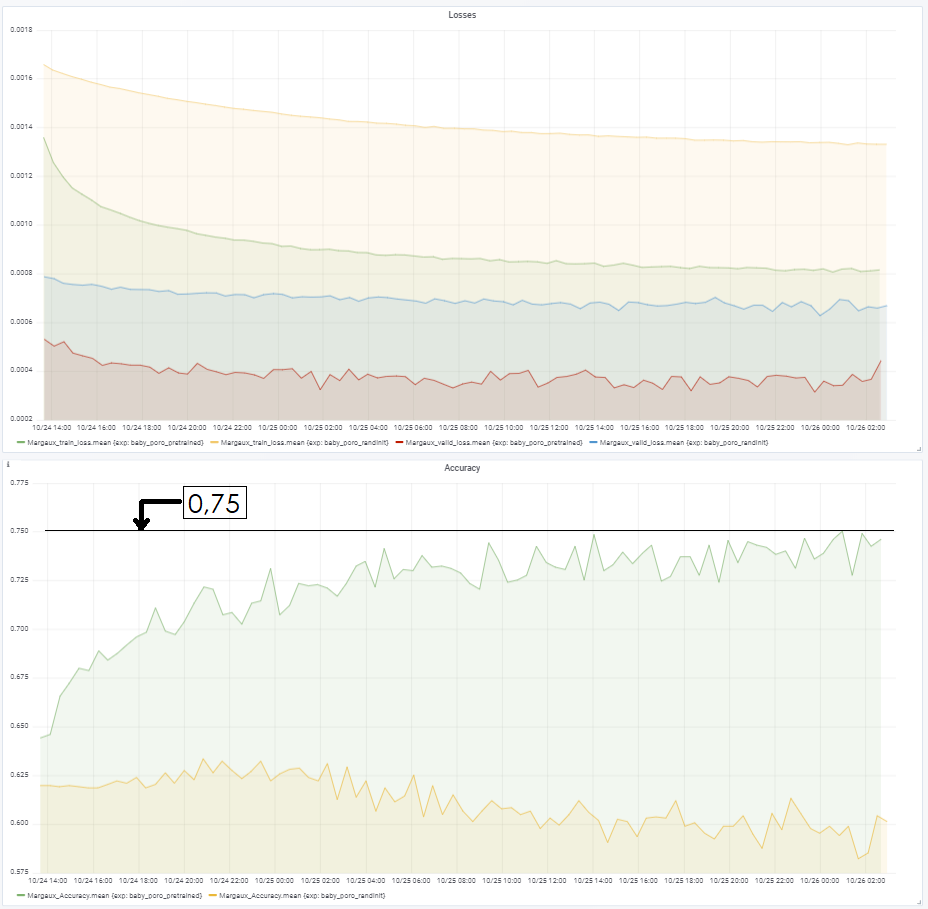
\includegraphics[width=.95\textwidth]{figures/04-Init_poro_acc.PNG}
\label{fig:resinit_poro}
\caption{ResNet 18 trained on the Porosity class.}
\end{subfigure}%
\begin{subfigure}[b]{.6\textwidth}
\centering
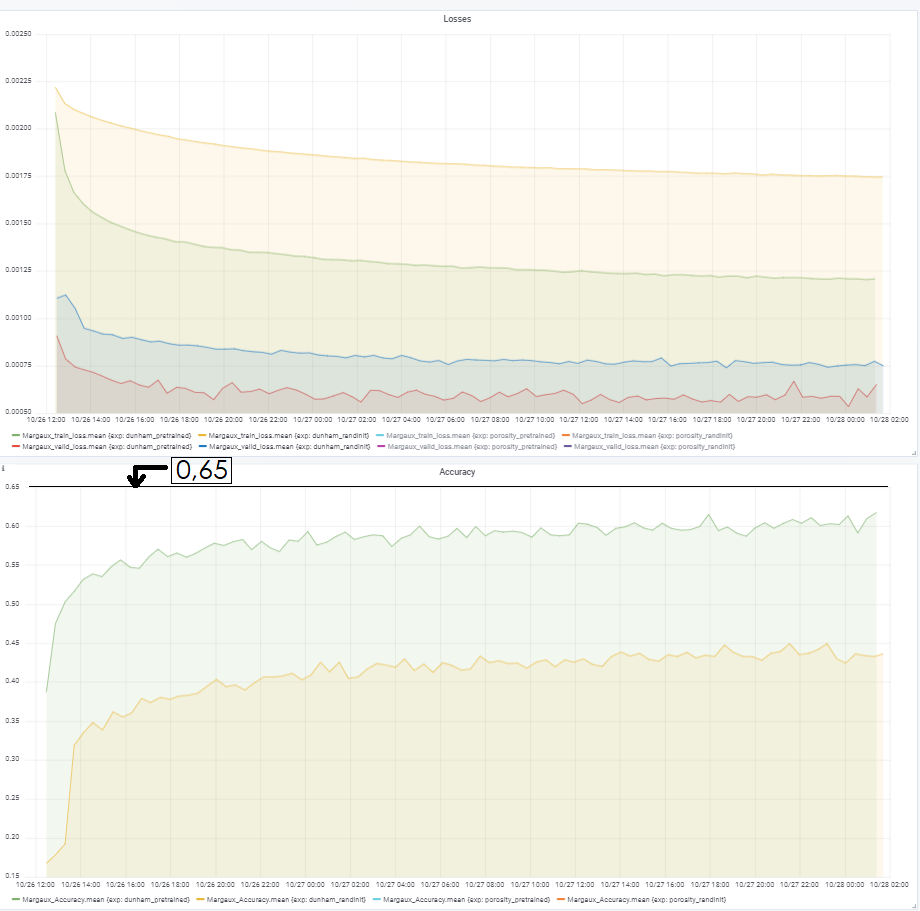
\includegraphics[width=.95\textwidth]{figures/04-Init_dunham_acc.PNG}
\label{fig:resinit_dunham}
\caption{ResNet 18 trained on the Dunham class.}
\end{subfigure}%
}\\
\makebox[\linewidth][c]{%
\begin{subfigure}[b]{.6\textwidth}
\centering
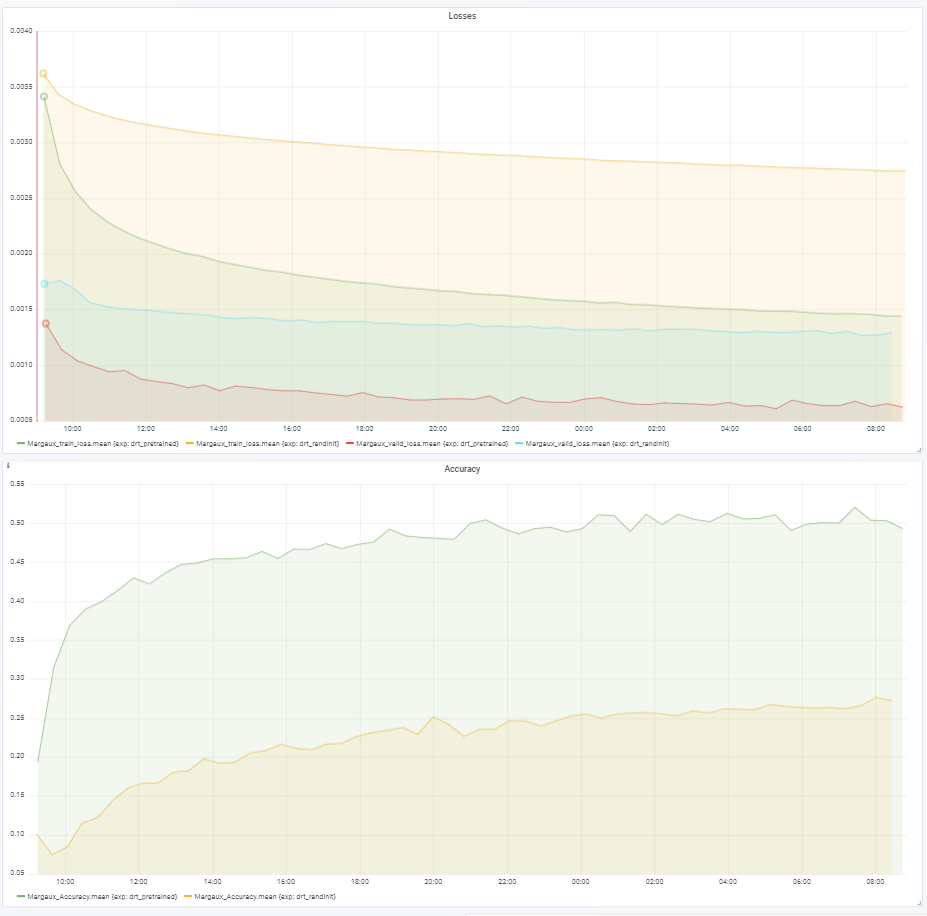
\includegraphics[width=.95\textwidth]{figures/04-Init_drt_acc.PNG}
\label{fig:resinit_drt}
\caption{ResNet 18 trained on the DRT class.}
\end{subfigure}%
\begin{subfigure}[b]{.6\textwidth}
\centering
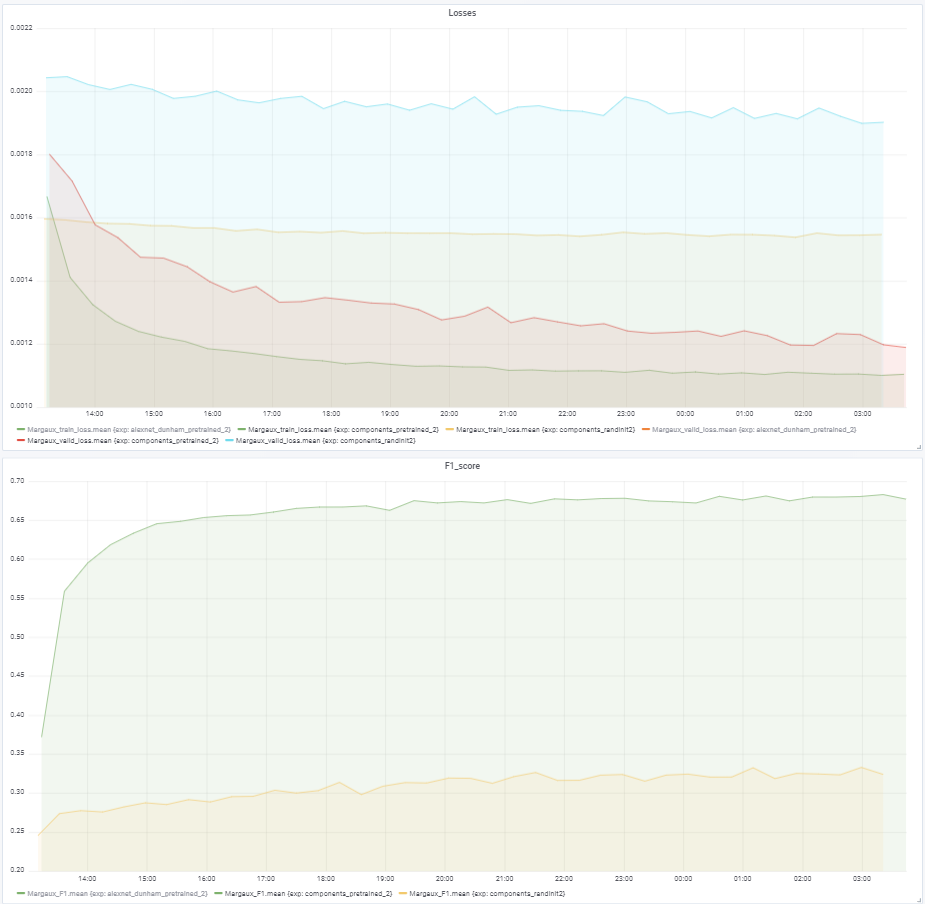
\includegraphics[width=.95\textwidth]{figures/04-Init_components_acc.PNG}
\label{fig:resinit_comp}
\caption{ResNet 18 trained on the Components class.}
\end{subfigure}%
}
\caption[Training and validation plots for ResNet 18]{The lines in green and red are for pretrained weights and yellow and blue for random initialization. The top plot is the validation accuracy for plots (a) (b) and (c) and the F1-score for plot (d), and the bottom plot is training  and validation loss.}
\label{fig:plotres}
\end{figure}

\subsection{Classification}
In Table \ref{tab:resbest}, we summarize the best validation and test accuracy or F-1 score for every class. Then we present the confusion matrix for the best performing model and the test data set for the single label classification in Figure \ref{fig:rescm}. For the Components class, we show the statistics for every class in Figure \ref{fig:perf_res}. 

\begin{table}
\caption{\label{tab:resbest} The results of the best version of the Resnet 18 on the classification task. The validation and test accuracy are used as score on the single label classification while F1-scores are used for multi-label classification.}
\centering
\begin{tabular}[b]{| l | l | l | l | l |}
\hline
    Initialization & Class & Validation score & Test score \ \\ \hline
    Pretrained Weights & Dunham &  60,7\%  & 37,3\% \\ \hline
    Pretrained Weights & Porosity & 73,8\%  &  58,5\% \\ \hline
    Pretrained Weights &DRT & 52,1\% &  22,1\% \\ \hline
    Pretrained Weights &Components & 69,1\% &  44,7\% \\ \hline
\end{tabular} 
\end{table}

\begin{figure}
\makebox[\linewidth][c]{%
\begin{subfigure}[b]{.6\textwidth}
\centering
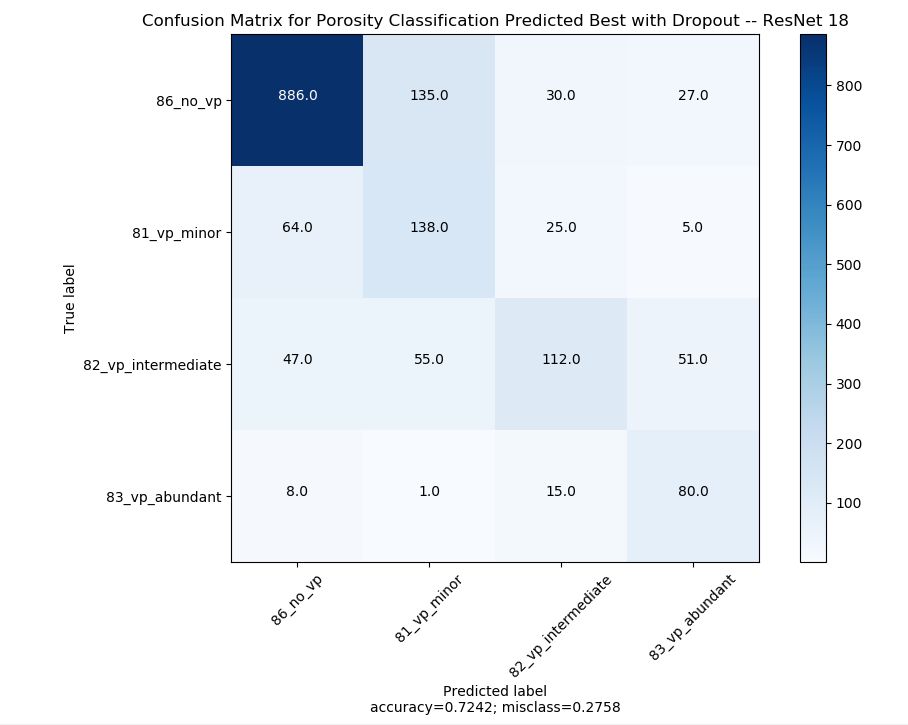
\includegraphics[width=.95\textwidth]{figures/04-baby_best.PNG}
\label{fig:rescm_poro}
\caption{Best for the Porosity class.}
\end{subfigure}%
\begin{subfigure}[b]{.6\textwidth}
\centering
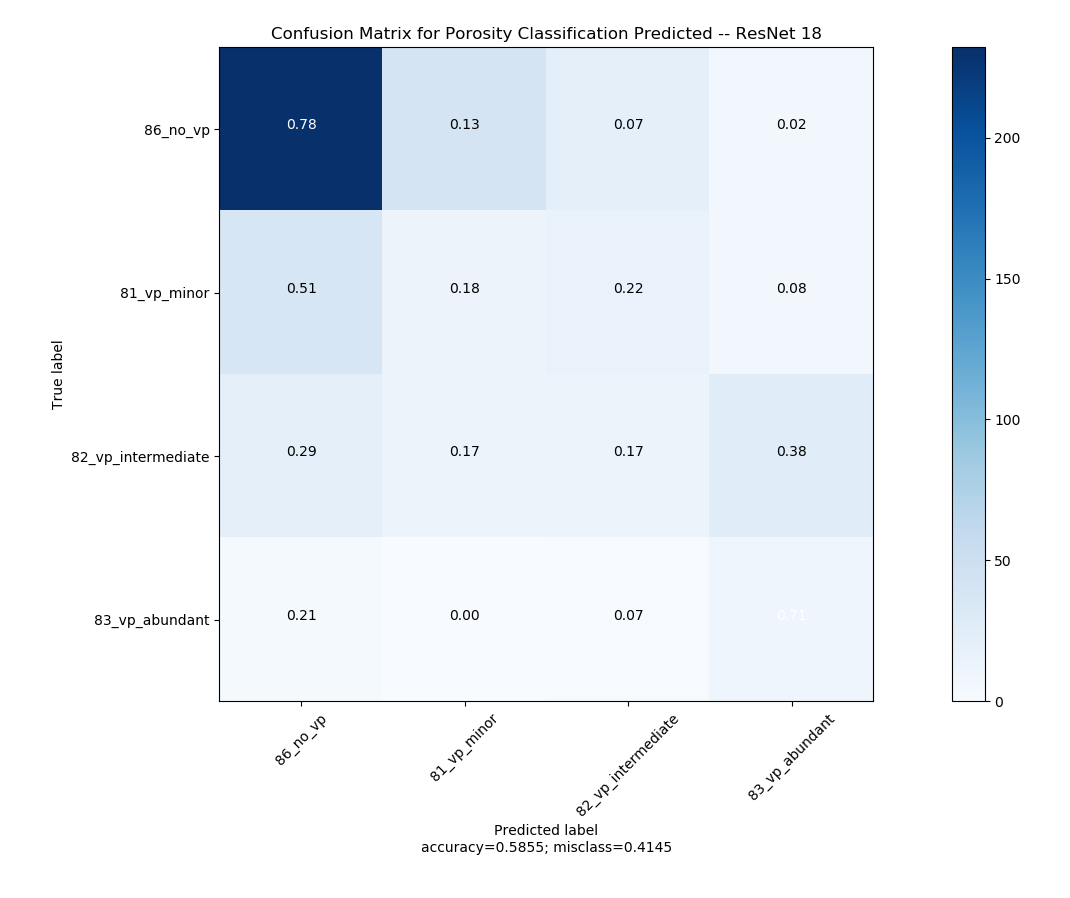
\includegraphics[width=.95\textwidth]{figures/04-baby_pred.PNG}
\label{fig:rescm_poro_pred}
\caption{Predicted for the Porosity class.}
\end{subfigure}%
}\\
\makebox[\linewidth][c]{%
\begin{subfigure}[b]{.6\textwidth}
\centering
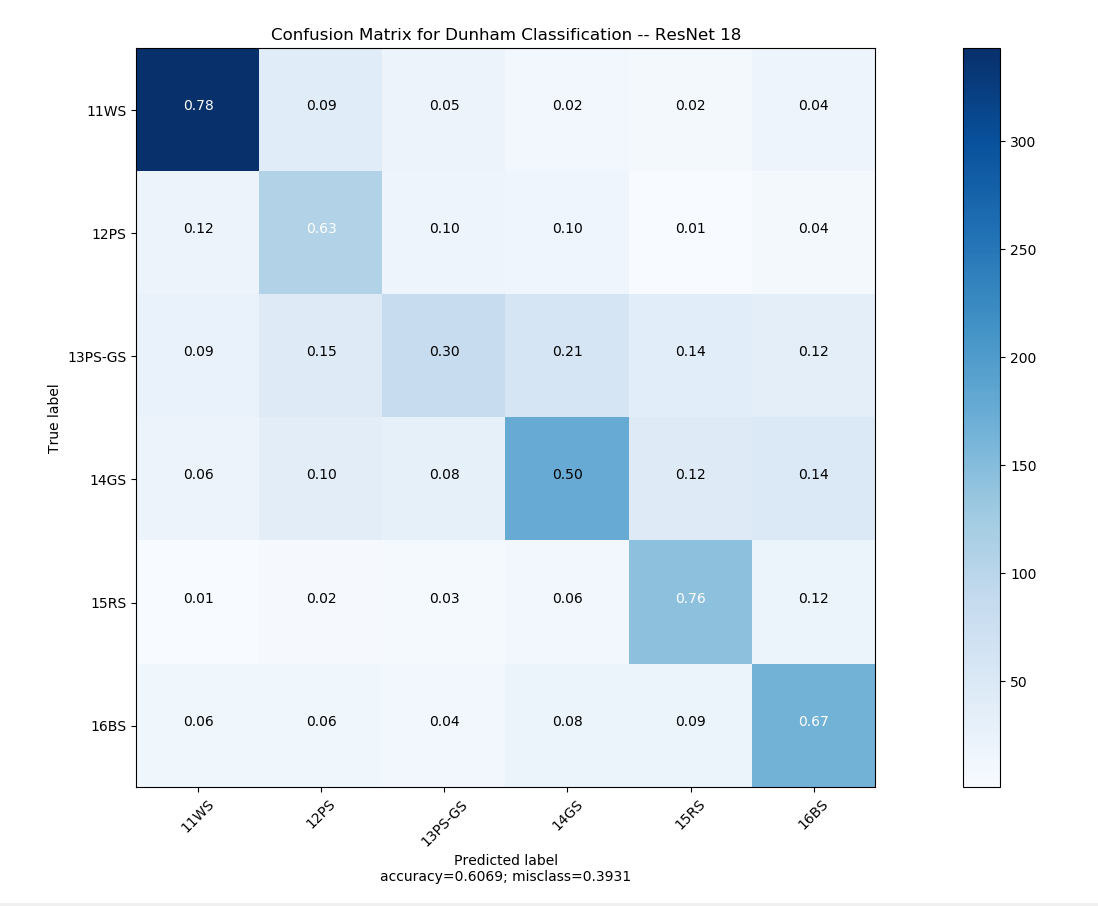
\includegraphics[width=.95\textwidth]{figures/04-dunham_best.PNG}
\label{fig:rescm_dunham}
\caption{Best for the Dunham class.}
\end{subfigure}%
\begin{subfigure}[b]{.6\textwidth}
\centering
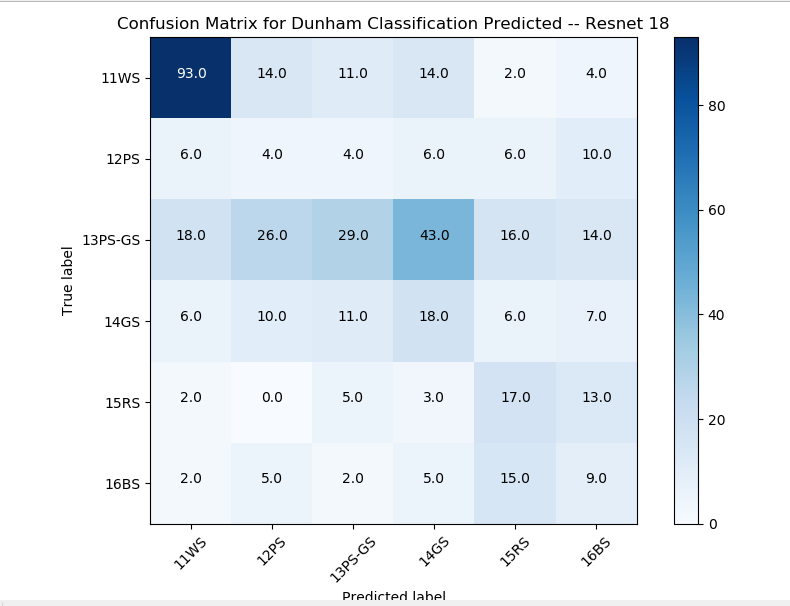
\includegraphics[width=.95\textwidth]{figures/04-dunham_pred.PNG}
\label{fig:rescm_dunham_pred}
\caption{Predicted for the Dunham class.}
\end{subfigure}%
}
\makebox[\linewidth][c]{%
\begin{subfigure}[b]{.6\textwidth}
\centering
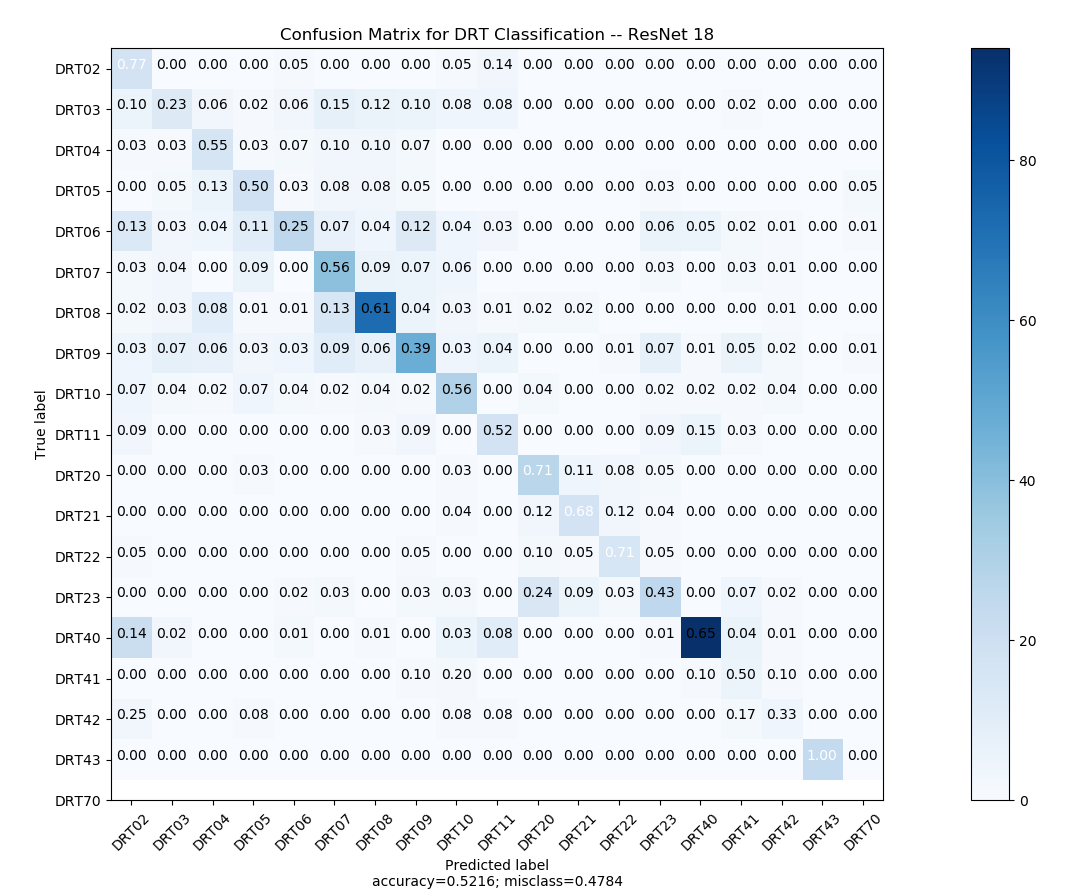
\includegraphics[width=.95\textwidth]{figures/04-drt_best.PNG}
\label{fig:rescm_drt}
\caption{Best for the DRT class.}
\end{subfigure}%
\begin{subfigure}[b]{.6\textwidth}
\centering
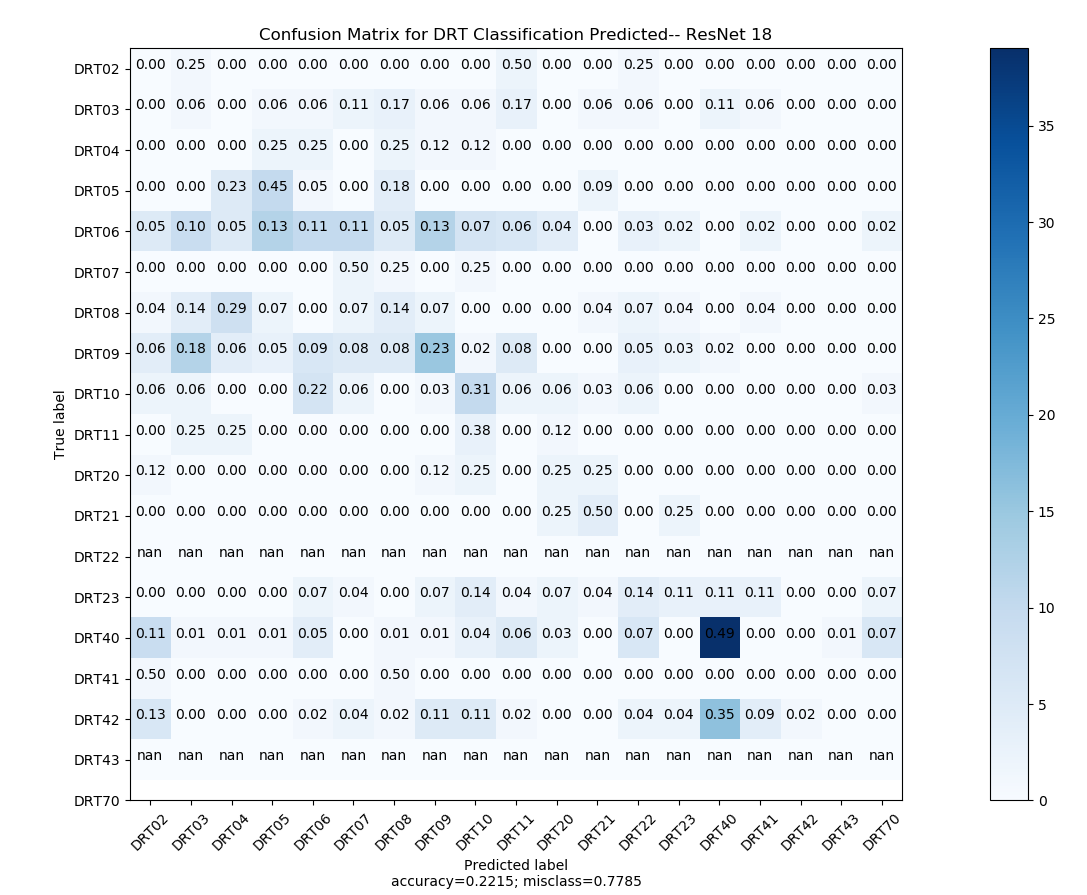
\includegraphics[width=.95\textwidth]{figures/04-drt_pred.PNG}
\label{fig:rescm_drt_pred}
\caption{Predicted for the DRT class.}
\end{subfigure}%
}
\caption[Confusion matrices of classes trained on Resnet 18]{On the left is the confusion matrix of the best performing ResNet18 and on the right is the confusion matrix on the test set.}
\label{fig:rescm}
\end{figure}

\begin{figure}
\makebox[\linewidth][c]{%
\begin{subfigure}[b]{.6\textwidth}
\centering
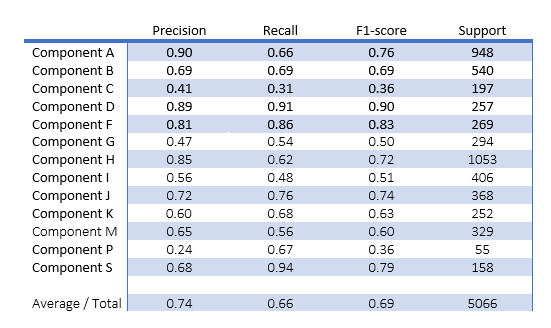
\includegraphics[width=.95\textwidth]{figures/04-compo_best.PNG}
\label{fig:rescm_comp}
\caption{Best for the Components class.}
\end{subfigure}%
\begin{subfigure}[b]{.6\textwidth}
\centering
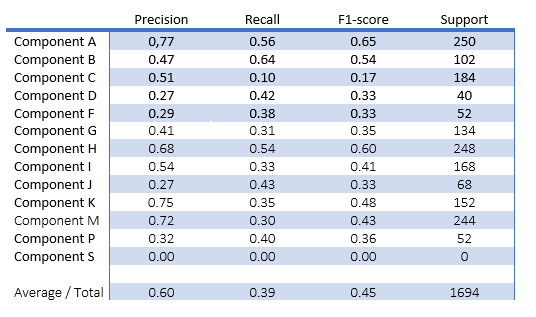
\includegraphics[width=.95\textwidth]{figures/04-compo_pred.PNG}
\label{fig:rescm_comp_pred}
\caption{Predicted for the Components class.}
\end{subfigure}%
}
\caption [Performance summary of the Components class trained on Resnet 18]{These figure are the summaries of the performance for the multi-label classification. It shows precision, recall f1-score and also the number of samples for each class.}
\label{fig:perf_res}
\end{figure}


%%%%%%%%%%%%%%%%%%%%%%%%%%%%%%%%%%%%%%%%%%%%%%%%%%%   ALEX   %%%%%%%%%%%%%%%%%%%%%%%%%%%%%%%%%%%%%%%%%%%%%%%%%%%%%

\section{AlexNet}\label{sec:aleX}
\subsection{Initialization}
For every class, we tested our network with either random initialization or with using pretrained weights. In Table \ref{tab:alexinit}, we can see the best accuracy on validation and test set, the number of epochs for training for each class.  
In Figure \ref{fig:plotsalex}, we plotted the accuracy, F1 score, and average training and validation loss for each class. 
\begin{table}
\caption{\label{tab:alexinit} The results of training AlexNet using random initialization or pretrained weights with Adamax as optimizer}
\centering
\begin{tabular}[b]{| l | l | l | l | l |}
\hline
    Initialization & Class & Validation accuracy  & Epochs\\ \hline
    \multirow{4}{*}{Pretrained Weights} & Dunham &  81,7\%  & 50 \\ %%cf Confusion Matrix 
    & Porosity & 88,5\% &  50 \\
    &DRT & 74,5\% &  50 \\
    &Components & 85,1\% &  50 \\ \hline
     \multirow{4}{*}{Random} & Dunham &  62,1\% & 50 \\
    & Porosity & 64,8\% &  50 \\
    &DRT & 60,7\% &  50 \\
    &Components & 72,3\% & 50 \\ \hline
\end{tabular} 
\end{table}

\begin{figure}
\makebox[\linewidth][c]{%
\begin{subfigure}[b]{.6\textwidth}
\centering
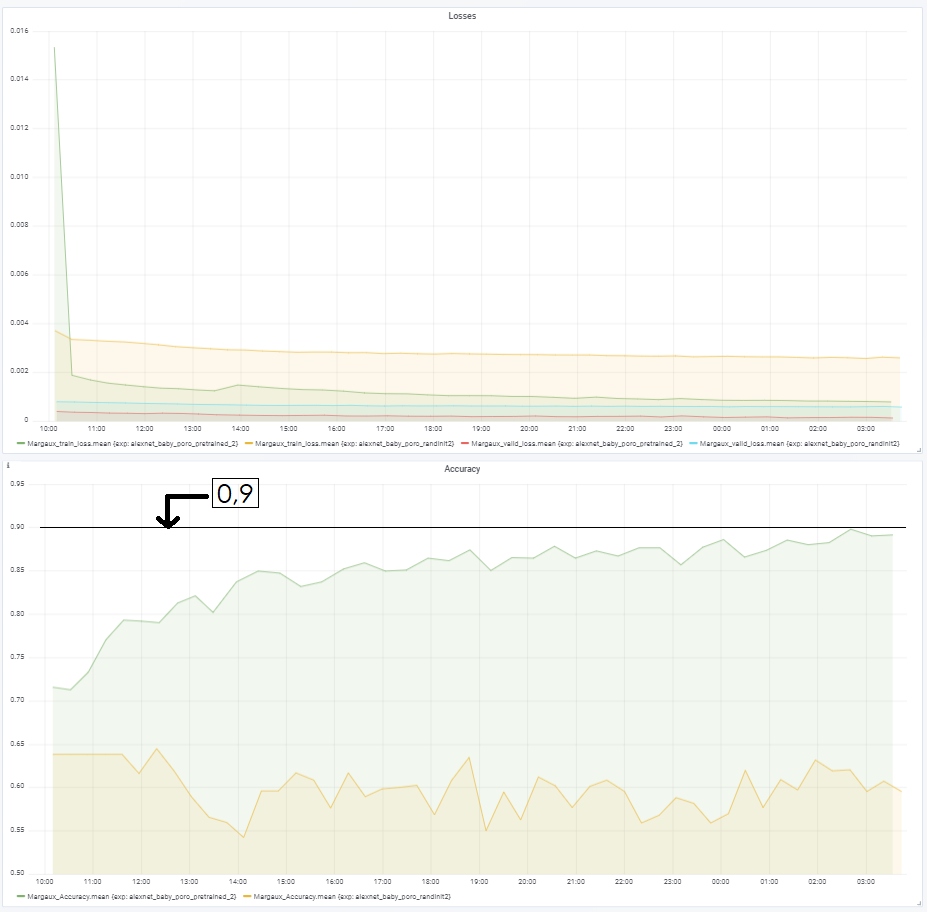
\includegraphics[width=.95\textwidth]{figures/04-Init_al_poro_acc.PNG}
\label{fig:alexinit_poro}
\caption{AlexNet trained on the Porosity class.}
\end{subfigure}%
\begin{subfigure}[b]{.6\textwidth}
\centering
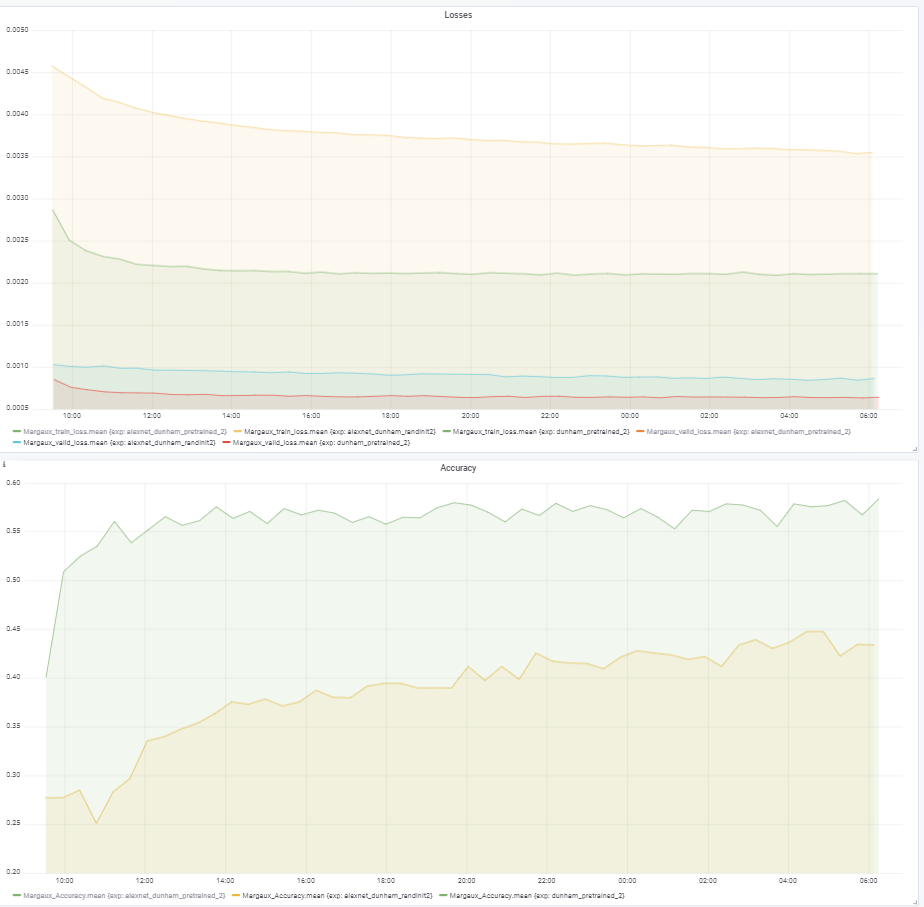
\includegraphics[width=.95\textwidth]{figures/04-Init_al_dunham_acc.PNG}
\label{fig:alexinit_dunham}
\caption{AlexNet trained on the Dunham class.}
\end{subfigure}%
}\\
\makebox[\linewidth][c]{%
\begin{subfigure}[b]{.6\textwidth}
\centering
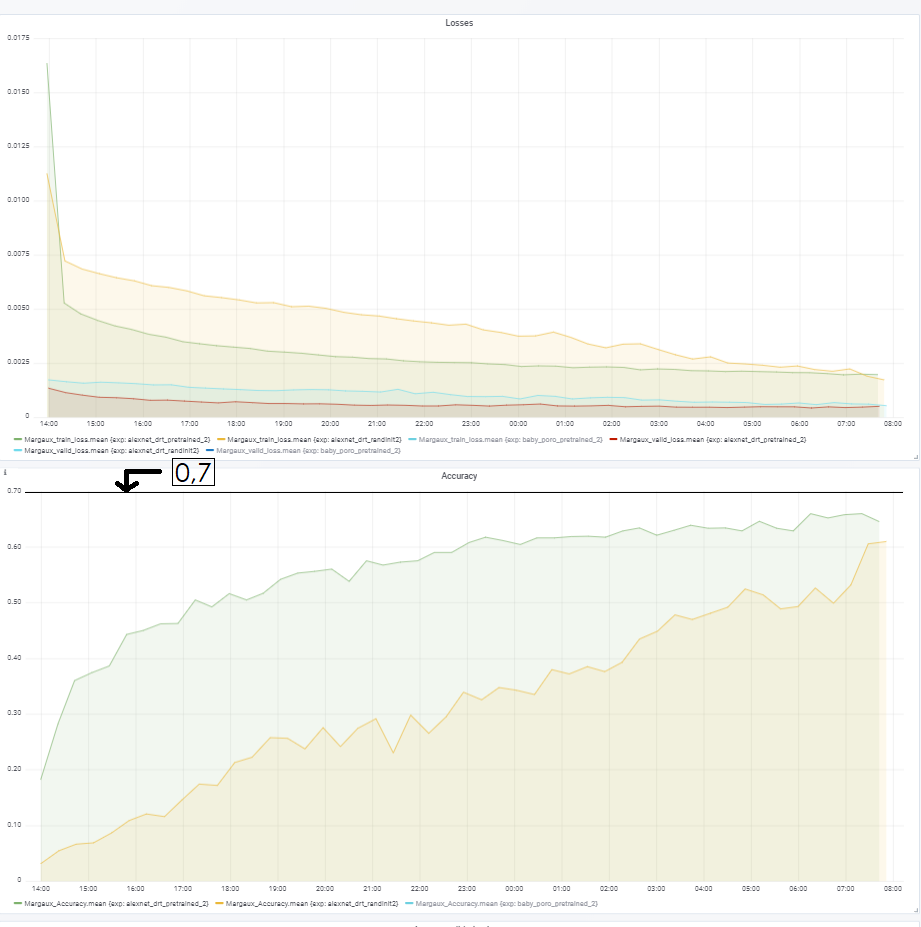
\includegraphics[width=.95\textwidth]{figures/04-Init_al_drt_acc.PNG}
\label{fig:alexinit_drt}
\caption{AlexNet trained on the DRT class.}
\end{subfigure}%
\begin{subfigure}[b]{.6\textwidth}
\centering
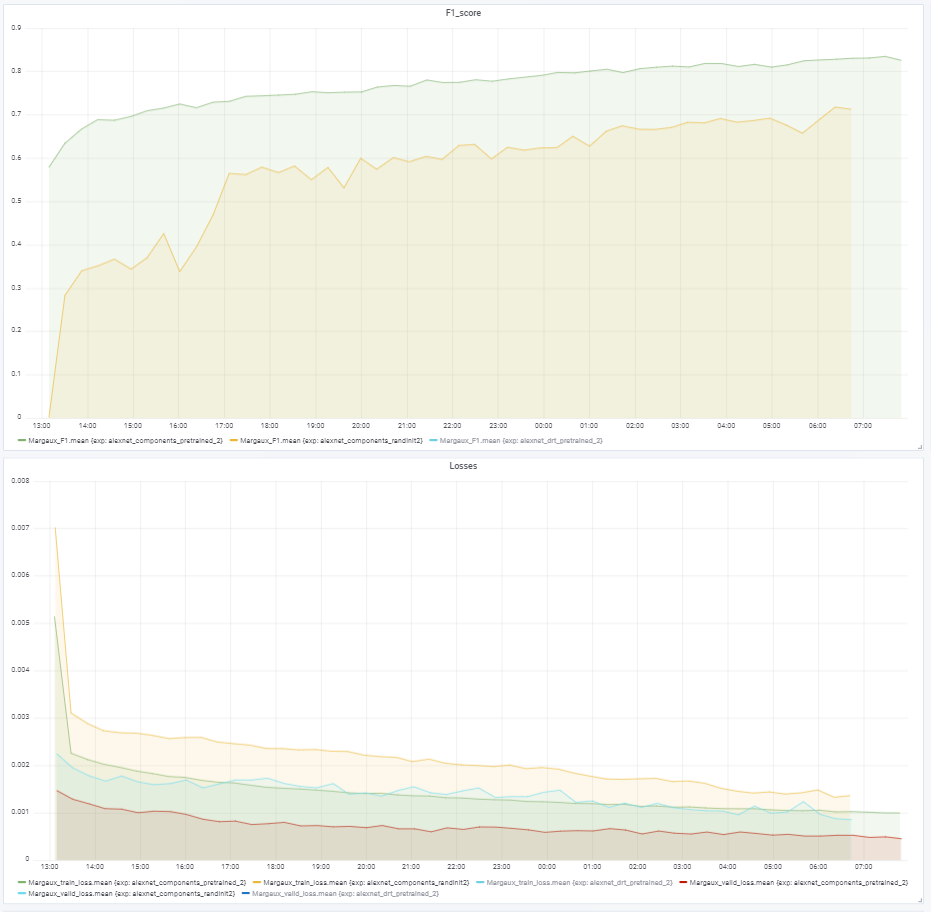
\includegraphics[width=.95\textwidth]{figures/04-al_components_acc.PNG}
\label{fig:alexinit_comp}
\caption{AlexNet trained on the Components class.}
\end{subfigure}%
}
\caption[Training and validation plots for AlexNet]{The lines in green and red are for pretrained weights and yellow and blue for random initialization. The top plot is the validation accuracy for plots (a) (b) and (c) and the F1-score for plot (d), and the bottom plot is training  and validation loss.}
\label{fig:plotsalex}
\end{figure}


\subsection{Classification}
In Table \ref{tab:alexbest}, we summarize the best validation and test accuracy or F-1 score for every class. Then we present the confusion matrix for the best performing model and the test data set for the single label classification on Figure \ref{fig:alcm}. For the Components class, we show the statistics for every class in Figure \ref{fig:perf_al}. 

\begin{table}
\caption{\label{tab:alexbest} The results of the best version of the AlexNet on the classification task. The validation and test accuracy are used as score on the single label classification while F1-scores are used for multi-label classification.}
\centering
\begin{tabular}[b]{| l | l | l | l | l |}
\hline
    Initialization & Class & Validation score & Test score  \\ \hline
    Pretrained Weights & Dunham &  81,7\%  & 36,8\% \\ \hline
    Pretrained Weights & Porosity & 88,5\%  &  69,5\% \\ \hline
    Pretrained Weights &DRT & 74,5\% &  23,4\% \\ \hline
    Pretrained Weights &Components & 85,1\% &  50,2\% \\ \hline
\end{tabular} 
\end{table}

\begin{figure}
\makebox[\linewidth][c]{%
\begin{subfigure}[b]{.6\textwidth}
\centering
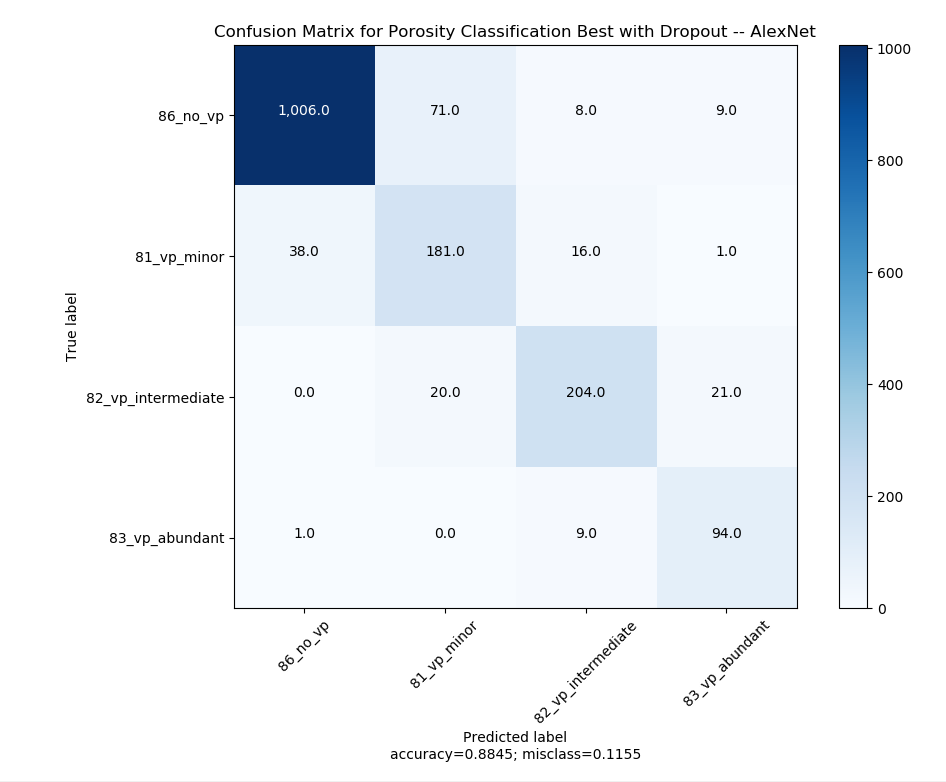
\includegraphics[width=.95\textwidth]{figures/04-al_baby_best.PNG}
\label{fig:alcm_poro}
\caption{Best for the Porosity class.}
\end{subfigure}%
\begin{subfigure}[b]{.6\textwidth}
\centering
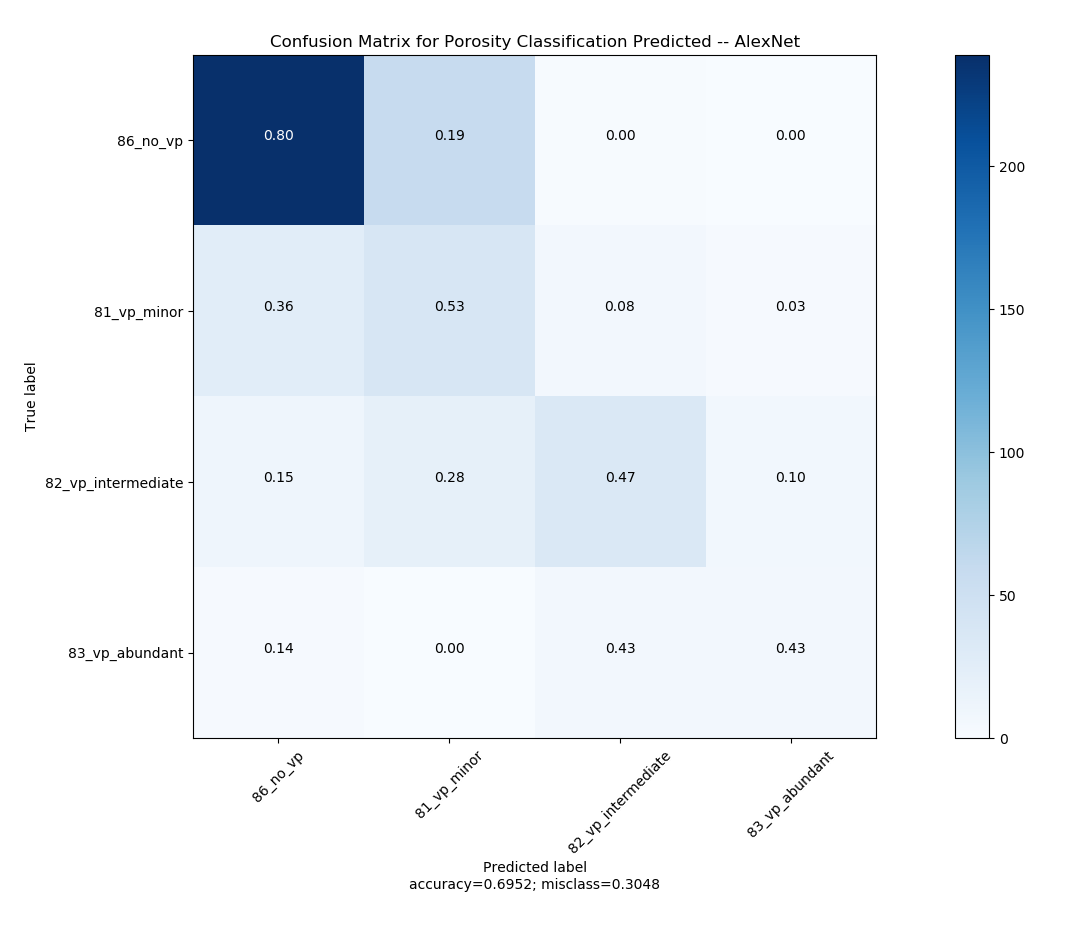
\includegraphics[width=.95\textwidth]{figures/04-al_baby_pred.PNG}
\label{fig:alcm_poro_pred}
\caption{Predicted for the Porosity class.}
\end{subfigure}%
}\\
\makebox[\linewidth][c]{%
\begin{subfigure}[b]{.6\textwidth}
\centering
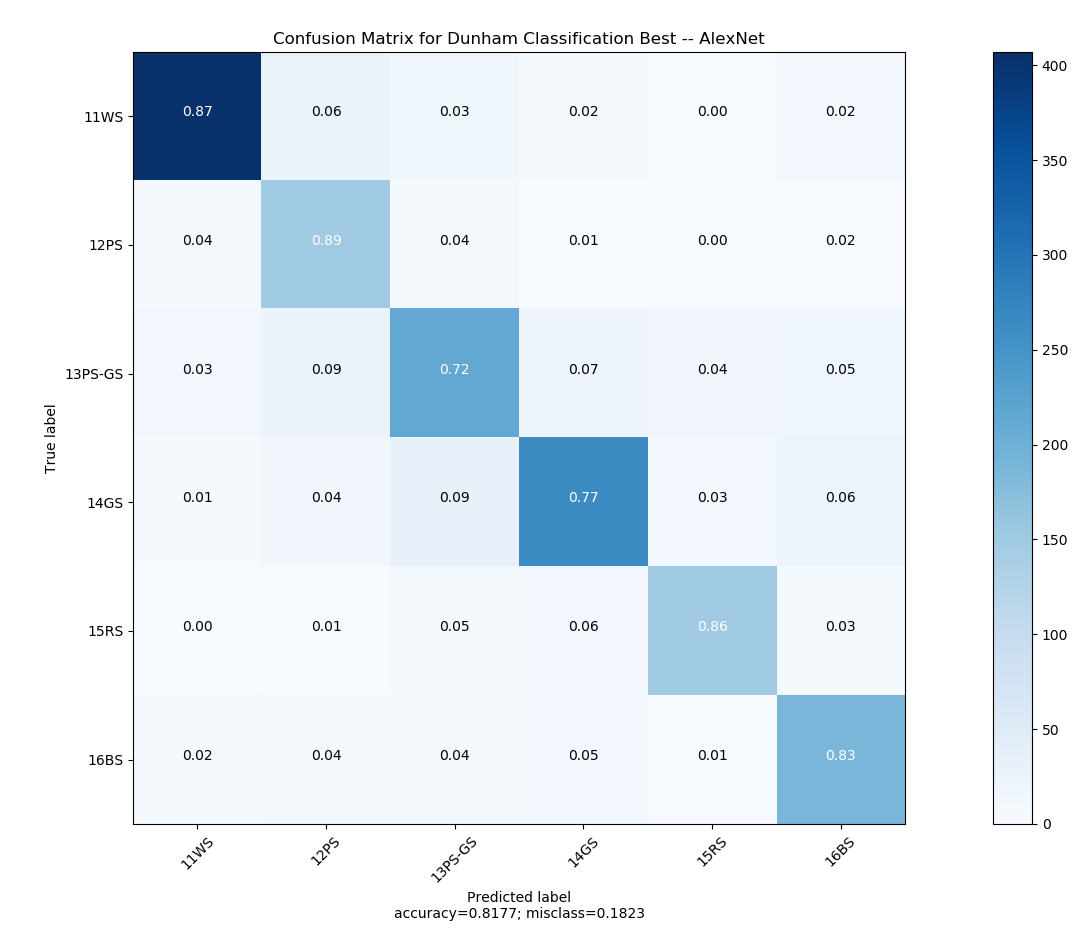
\includegraphics[width=.95\textwidth]{figures/04-al_dunham_best.PNG}
\label{fig:alcm_dunham}
\caption{Best for the Dunham class.}
\end{subfigure}%
\begin{subfigure}[b]{.6\textwidth}
\centering
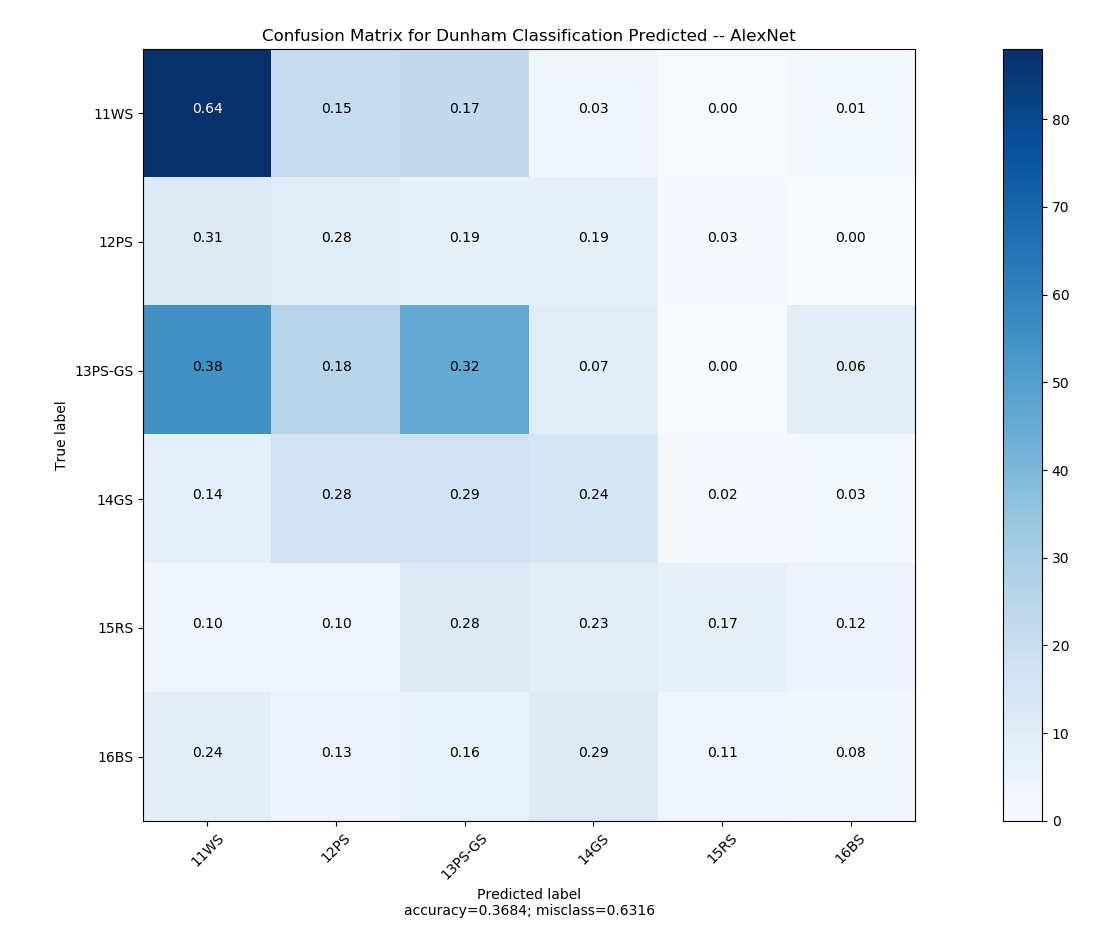
\includegraphics[width=.95\textwidth]{figures/04-al_dunham_pred.PNG}
\label{fig:alcm_dunham_pred}
\caption{Predicted for the Dunham class.}
\end{subfigure}%
}
\makebox[\linewidth][c]{%
\begin{subfigure}[b]{.6\textwidth}
\centering
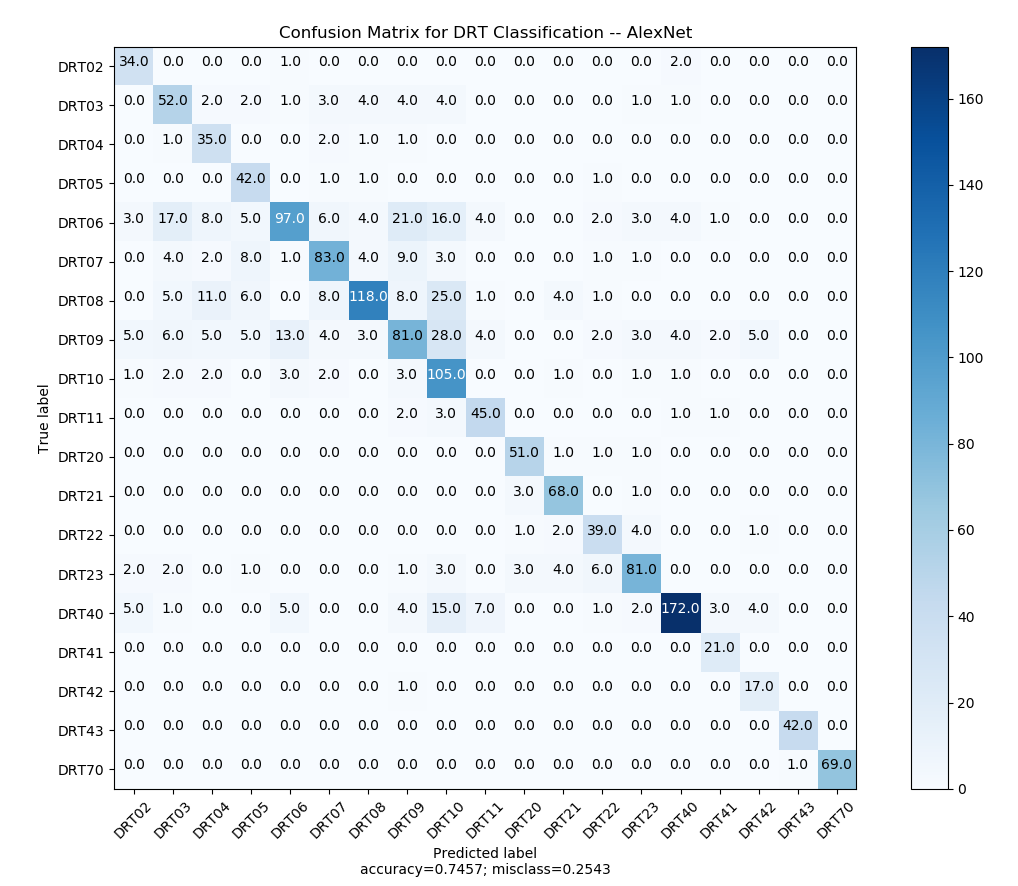
\includegraphics[width=.95\textwidth]{figures/04-al_drt_best.PNG}
\label{fig:alcm_drt}
\caption{Best for the DRT class.}
\end{subfigure}%
\begin{subfigure}[b]{.6\textwidth}
\centering
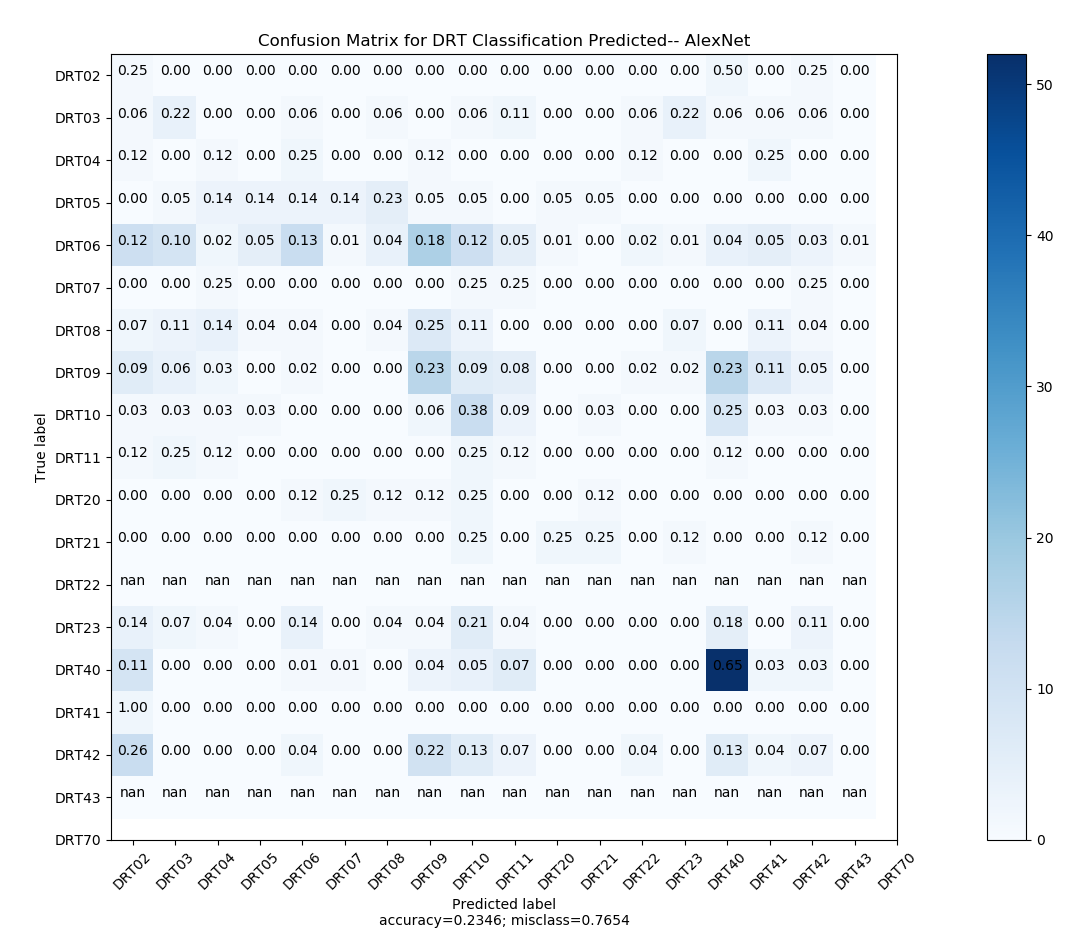
\includegraphics[width=.95\textwidth]{figures/04-al_drt_pred.PNG}
\label{fig:alcm_drt_pred}
\caption{Predicted for the DRT class.}
\end{subfigure}%
}
\caption[Confusion matrices of classes trained on AlexNet]{On the left is the confusion matrix of the best performing AlexNet and on the right is the confusion matrix on the test set.}
\label{fig:alcm}
\end{figure}

\begin{figure}
\makebox[\linewidth][c]{%
\begin{subfigure}[b]{.6\textwidth}
\centering
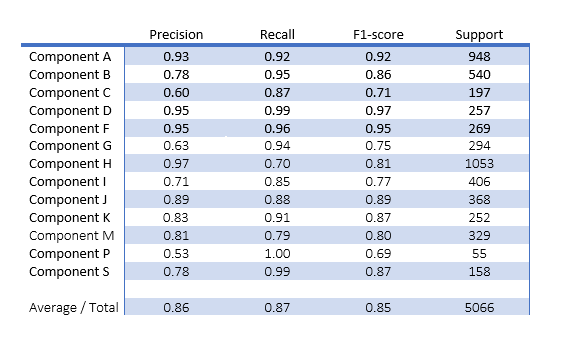
\includegraphics[width=.95\textwidth]{figures/04-al_compo_best.PNG}
\label{fig:alcm_comp}
\caption{Best for the Components class.}
\end{subfigure}%
\begin{subfigure}[b]{.6\textwidth}
\centering
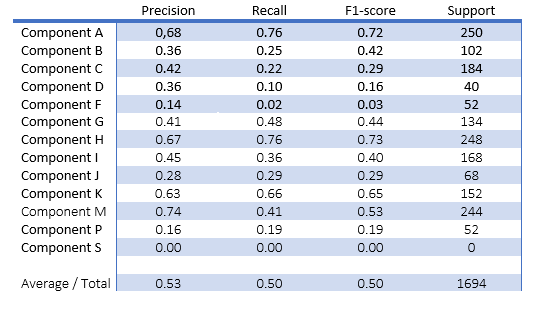
\includegraphics[width=.95\textwidth]{figures/04-al_compo_pred.PNG}
\label{fig:alcm_comp_pred}
\caption{Predicted for the Components class.}
\end{subfigure}%
}
\caption [Performance summary of the Components class trained on AlexNet]{These figure are the summaries of the performance for the multi-label classification trained on AlexNet. It shows precision, recall, f1-score and also the number of samples for each class.}
\label{fig:perf_al}
\end{figure}

%%%%%%%%%%%%%%%%%%%%%%%%%%%%%%%%%%%%%%%%%%%%%%%%%%%   GOOGLE   %%%%%%%%%%%%%%%%%%%%%%%%%%%%%%%%%%%%%%%%%%%%%%%%%%%


\section{Inception\_v3}\label{sec:gogl}
\subsection{Initialization}
For every class, we tested our network with either random initialization or with using pretrained weights. In Table \ref{tab:googinit}, we can see the best accuracy on validation and test set, the number of epochs for training for each class.  
In Figure \ref{fig:plotsgoogl}, we plotted the accuracy, F1 score, and average training and validation loss for each class. 

\begin{table}
\caption{\label{tab:googinit} The results of training Inception\_v3 network using random initialization or pretrained weights with Adamax as optimizer}
\centering
\begin{tabular}[b]{| l | l | l | l | l |}
\hline
    Initialization & Class & Validation score  & Epochs\\ \hline
    \multirow{4}{*}{Pretrained} & Dunham &  61,1\%  & 30 \\ %%cf Confusion Matrix 
    & Porosity & 76,1\% &  30 \\
    &DRT & 57,9\% &  30 \\
    &Components & 70,2\% &  50 \\ \hline
     \multirow{4}{*}{Random} & Dunham &  90,4\% & 30 \\
    & Porosity & 97,5\% &  30 \\
    &DRT & 99,2\% &  30 \\
    &Components & 96,3\% & 30 \\ \hline
\end{tabular} 
\end{table}

\begin{figure}
\makebox[\linewidth][c]{%
\begin{subfigure}[b]{.6\textwidth}
\centering
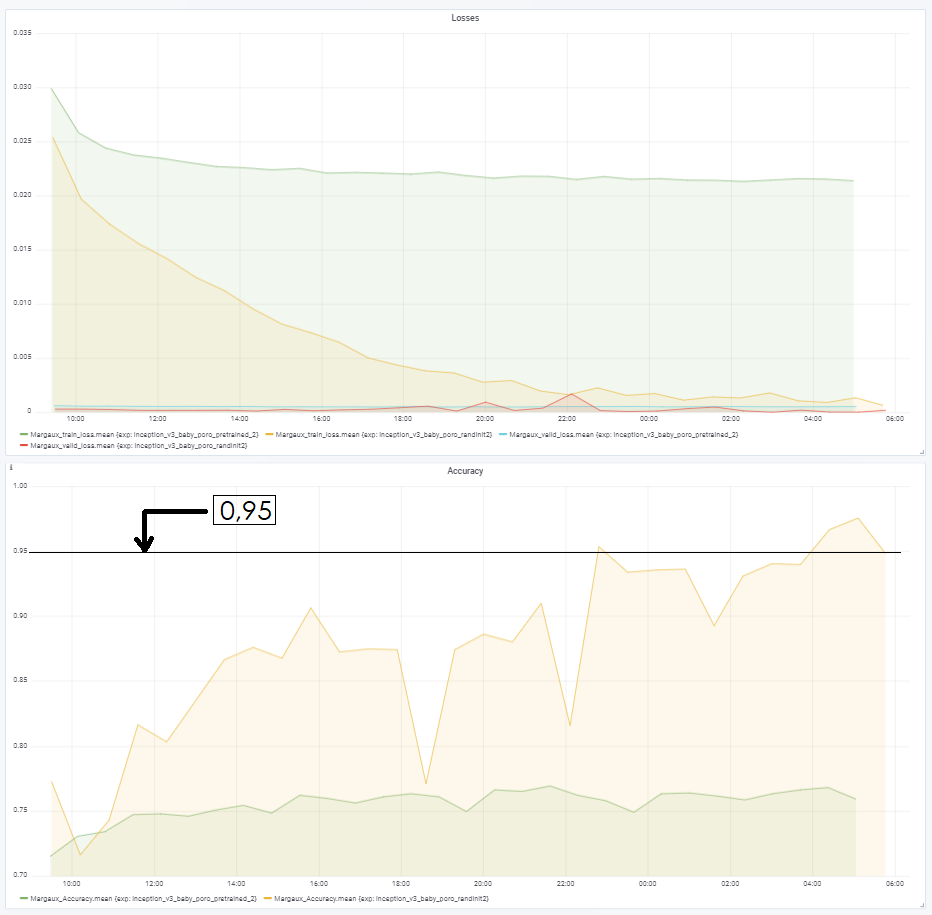
\includegraphics[width=.95\textwidth]{figures/04-go_poro_acc.PNG}
\label{fig:googinit_poro}
\caption{Inception\_v3 trained on the Porosity class.}
\end{subfigure}%
\begin{subfigure}[b]{.6\textwidth}
\centering
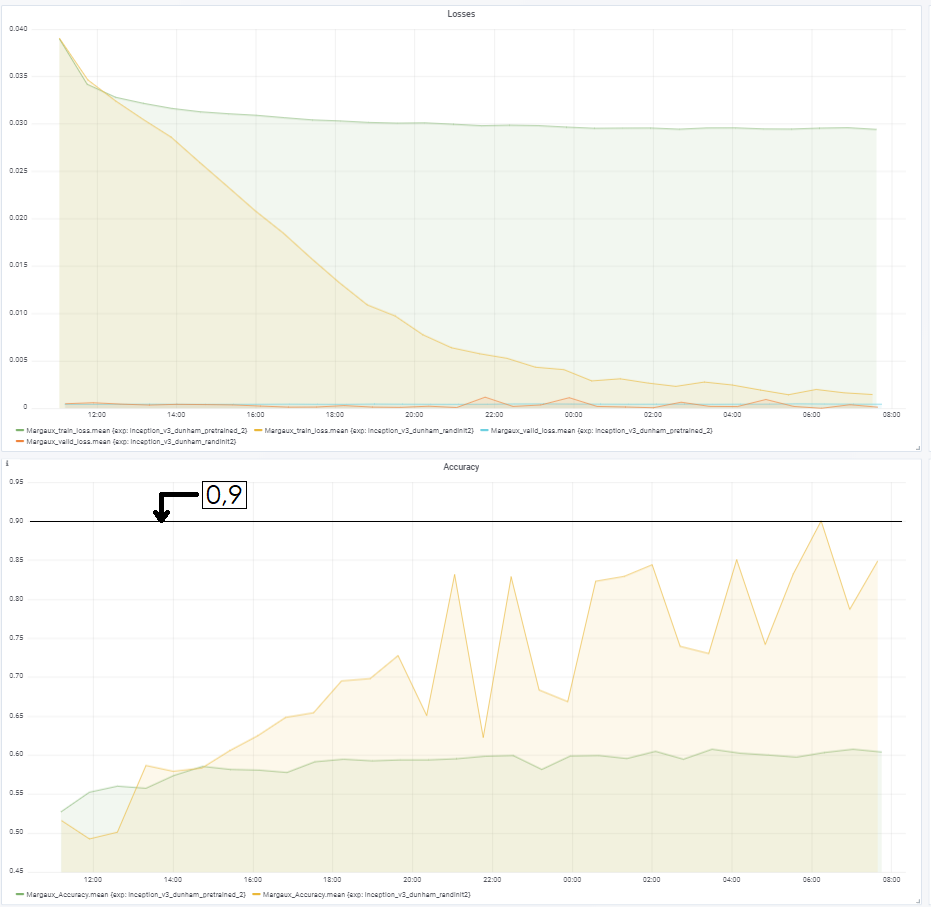
\includegraphics[width=.95\textwidth]{figures/04-go_dunham_acc.PNG}
\label{fig:googinit_dunham}
\caption{Inception\_v3 trained on the Dunham class.}
\end{subfigure}%
}\\
\makebox[\linewidth][c]{%
\begin{subfigure}[b]{.6\textwidth}
\centering
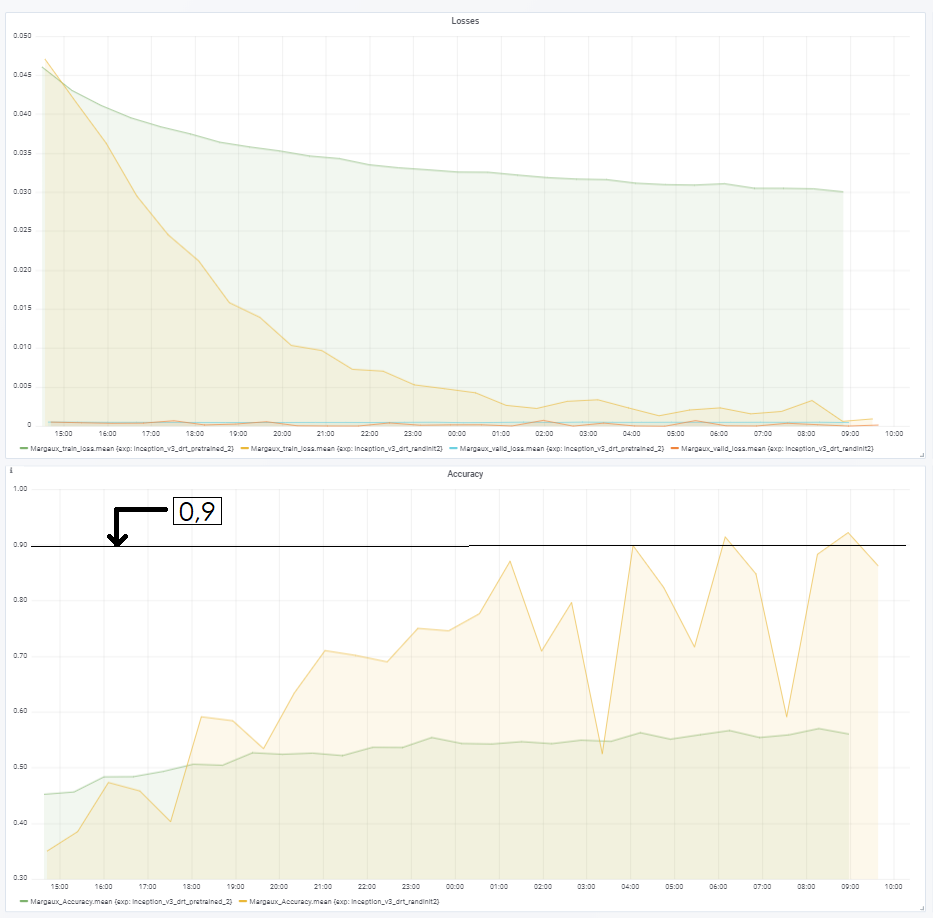
\includegraphics[width=.95\textwidth]{figures/04-go_drt_acc.PNG}
\label{fig:googinit_drt}
\caption{Inception\_v3 trained on the DRT class.}
\end{subfigure}%
\begin{subfigure}[b]{.6\textwidth}
\centering
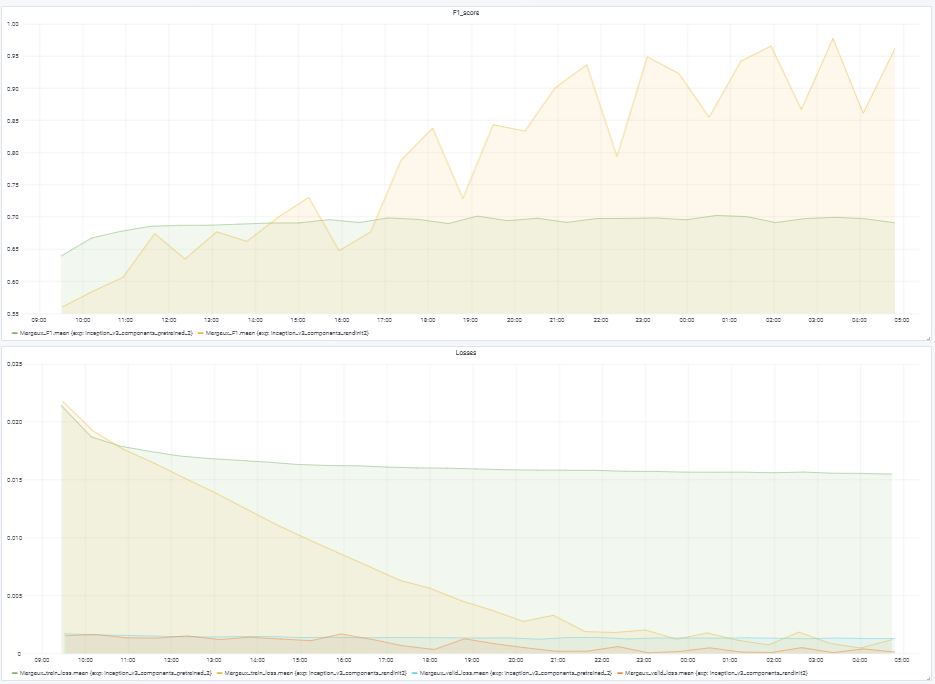
\includegraphics[width=.95\textwidth]{figures/04-go_conponents_acc.PNG}
\label{fig:googinit_comp}
\caption{Inception\_v3 trained on the Components class.}
\end{subfigure}%
}
\caption[Training and validation plots for Inception\_v3]{The lines in green and red are for pretrained weights and yellow and blue for random initialization. The top plot is the validation accuracy for plots (a) (b) and (c) and the F1-score for plot (d), and the bottom plot is training  and validation loss.}
\label{fig:plotsgoogl}
\end{figure}


\subsection{Classification}
In Table \ref{tab:googbest}, we summarize the best validation and test accuracy or F-1 score for every class. Then we present the confusion matrix for the best performing model and the test data set for the single label classification on Figure \ref{fig:gocm}. For the Components class, we show the statistics for every class in Figure \ref{fig:perf_goog}. 

\begin{table}
\caption{\label{tab:googbest} The results of the best version of the Inception\_v3 on the classification task. The validation and test accuracy are used as score on the single label classification while F1-scores are used for multi-label classification.}
\centering
\begin{tabular}[b]{| l | l | l | l | l |}
\hline
    Initialization & Class & Validation score & Test score \ \\ \hline
    Random & Dunham &  90,1\%  & 66,2\% \\ \hline
    Random & Porosity &  97,5\%  & 76,2\% \\ \hline
    Random &DRT & 99,2\% & 53,7\% \\ \hline
    Random &Components & 95,7\% &  44,6\% \\ \hline
\end{tabular} 
\end{table}

\begin{figure}
\makebox[\linewidth][c]{%
\begin{subfigure}[b]{.6\textwidth}
\centering
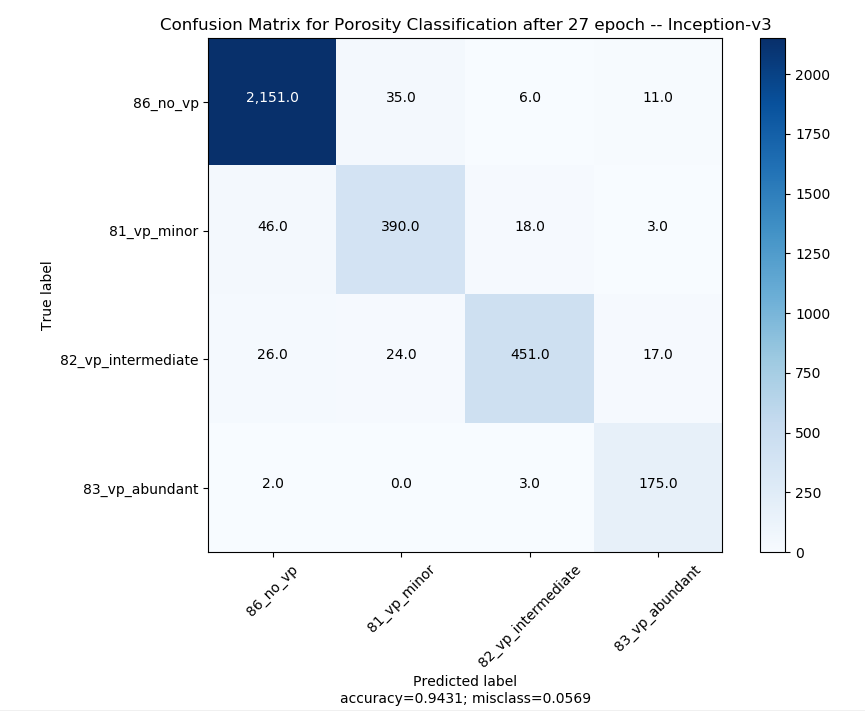
\includegraphics[width=.95\textwidth]{figures/04-go_baby_best.PNG}
\label{fig:gocm_poro}
\caption{Best for the Porosity class.}
\end{subfigure}%
\begin{subfigure}[b]{.6\textwidth}
\centering
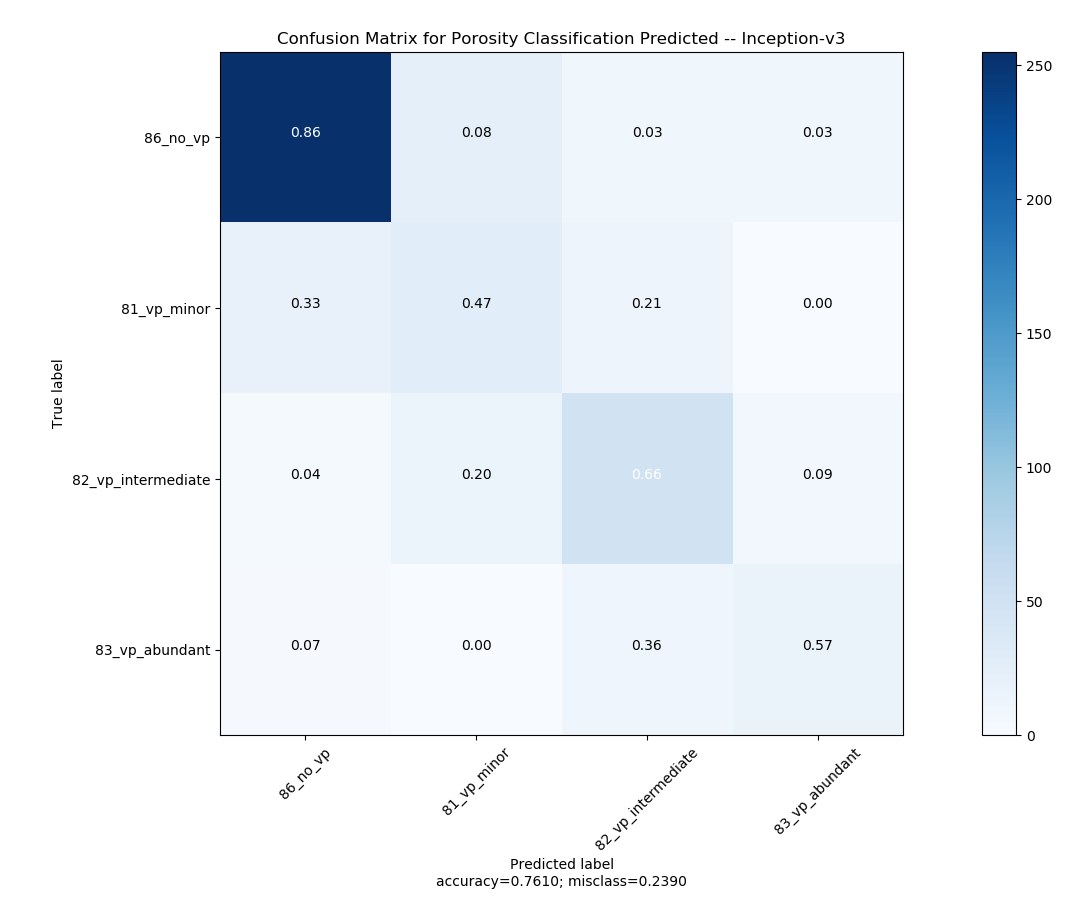
\includegraphics[width=.95\textwidth]{figures/04-go_baby_pred.PNG}
\label{fig:gocm_poro_pred}
\caption{Predicted for the Porosity class.}
\end{subfigure}%
}\\
\makebox[\linewidth][c]{%
\begin{subfigure}[b]{.6\textwidth}
\centering
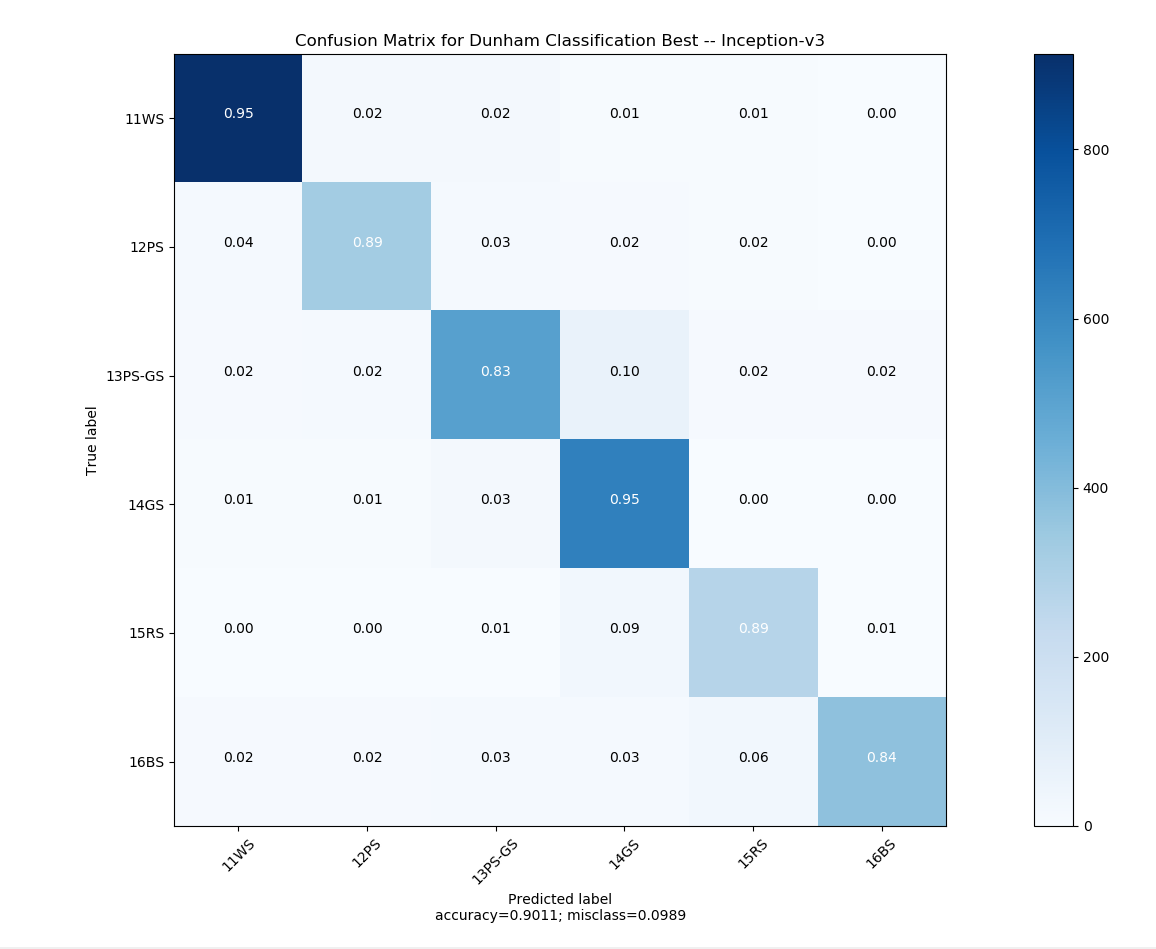
\includegraphics[width=.95\textwidth]{figures/04-go_dunham_best.PNG}
\label{fig:gocm_dunham}
\caption{Best for the Dunham class.}
\end{subfigure}%
\begin{subfigure}[b]{.6\textwidth}
\centering
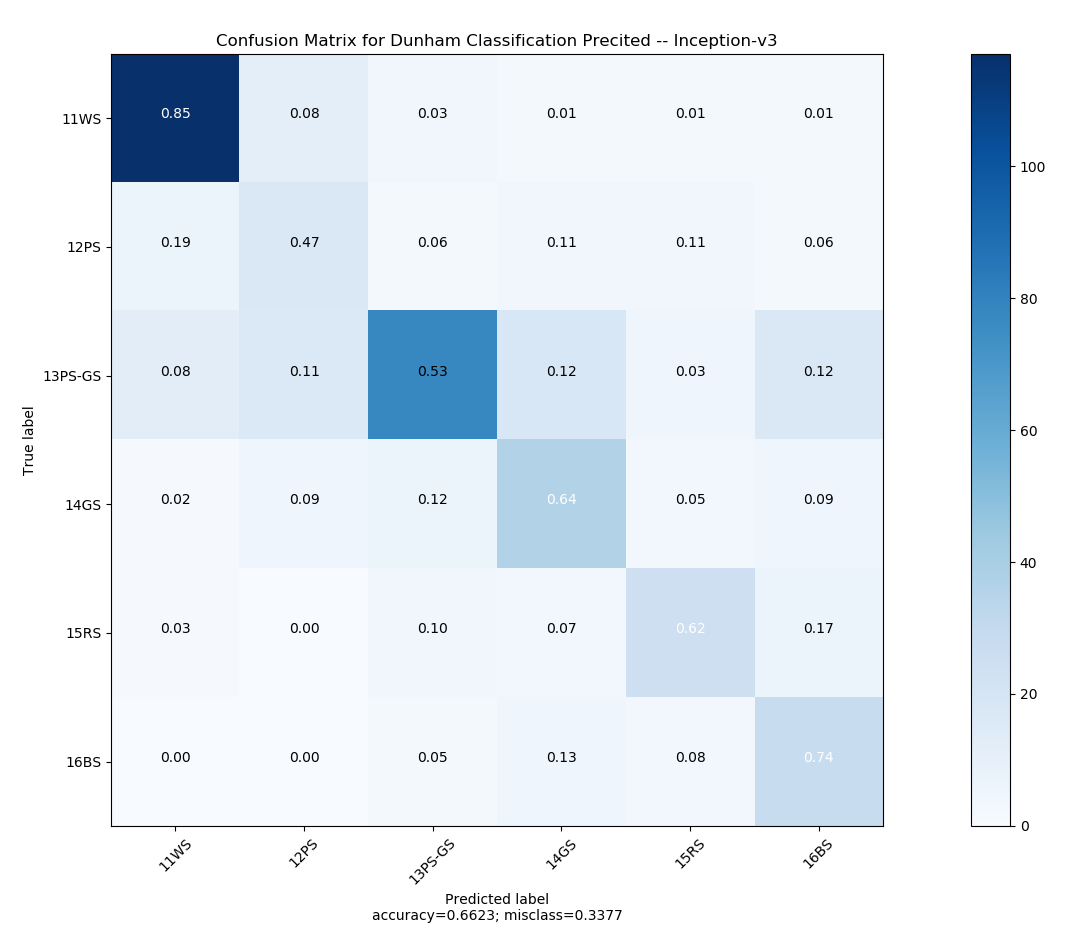
\includegraphics[width=.95\textwidth]{figures/04-go_dunham_pred.PNG}
\label{fig:gocm_dunham_pred}
\caption{Predicted for the Dunham class.}
\end{subfigure}%
}
\makebox[\linewidth][c]{%
\begin{subfigure}[b]{.6\textwidth}
\centering
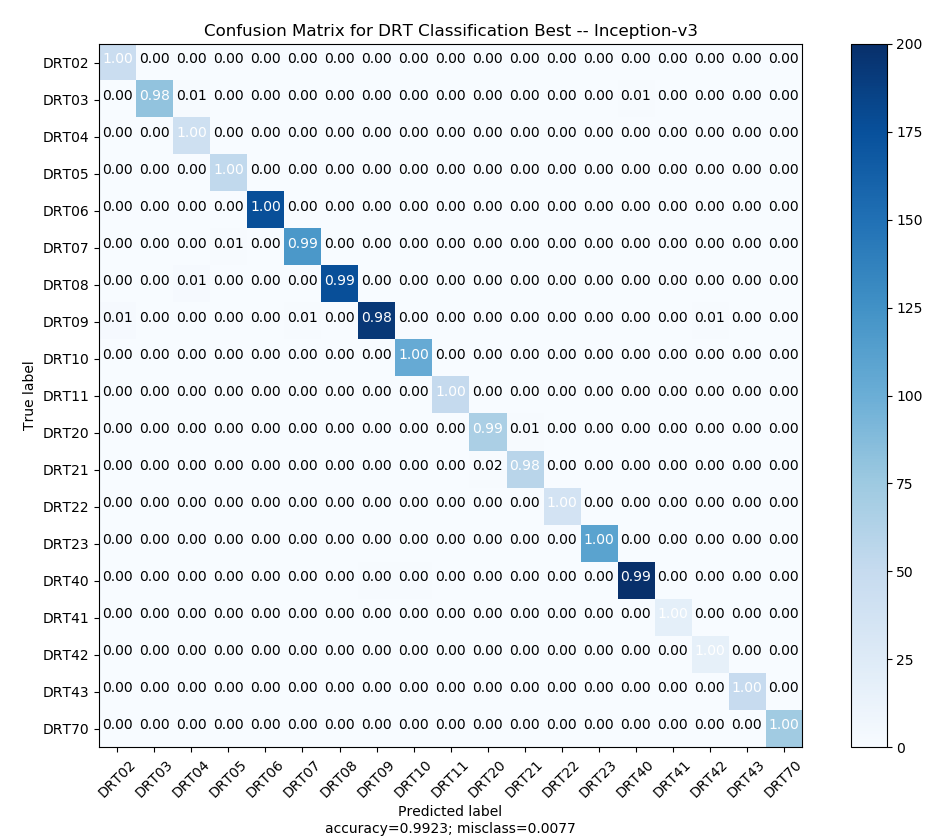
\includegraphics[width=.95\textwidth]{figures/04-go_drt_best.PNG}
\label{fig:gocm_drt}
\caption{Best for the DRT class.}
\end{subfigure}%
\begin{subfigure}[b]{.6\textwidth}
\centering
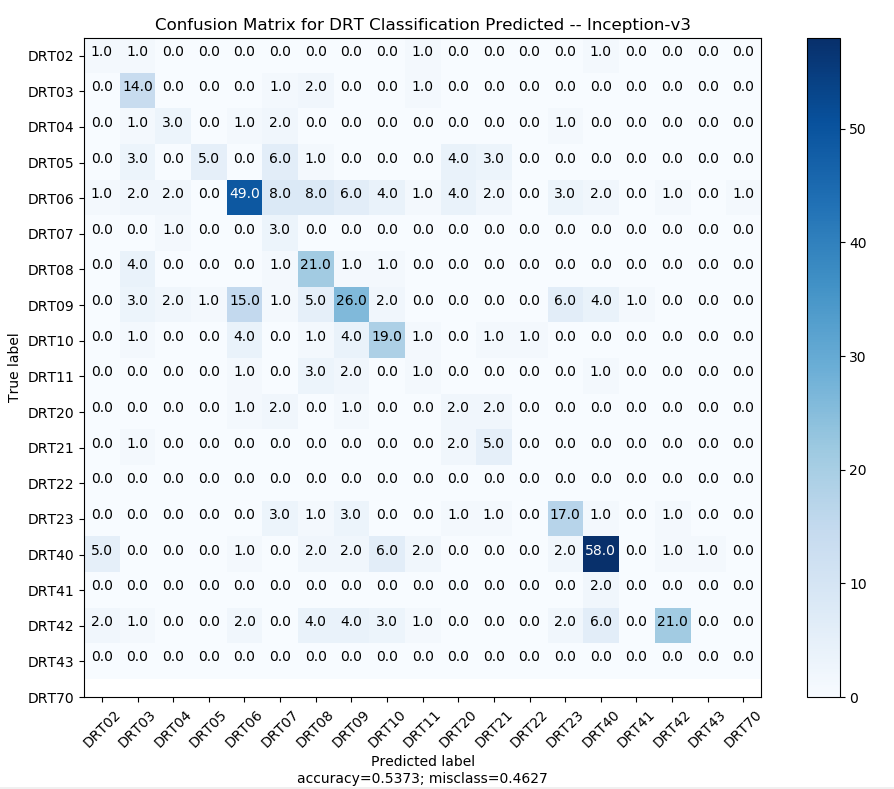
\includegraphics[width=.95\textwidth]{figures/04-go_drt_pred.PNG}
\label{fig:gocm_drt_pred}
\caption{Predicted for the DRT class.}
\end{subfigure}%
}
\caption[Confusion matrices of classes trained on Inception\_v3]{On the left is the confusion matrix of the best performing Inception\_v3 and on the right is the confusion matrix on the test set.}
\label{fig:gocm}
\end{figure}

\begin{figure}
\makebox[\linewidth][c]{%
\begin{subfigure}[b]{.6\textwidth}
\centering
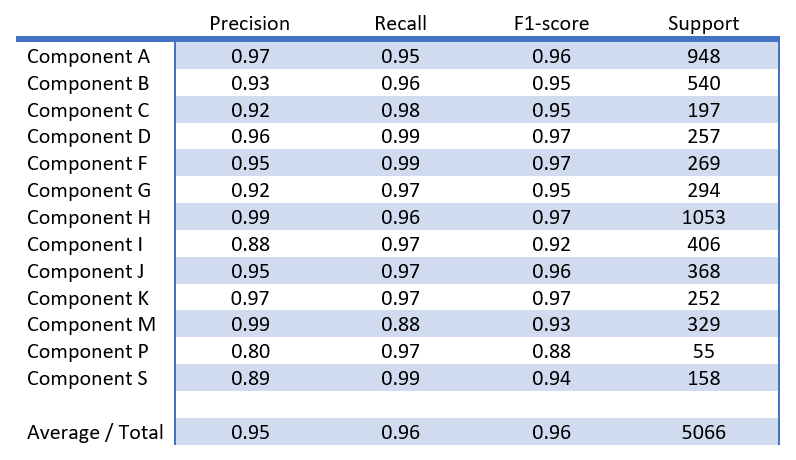
\includegraphics[width=.95\textwidth]{figures/04-go_compo_best.PNG}
\label{fig:gocm_comp}
\caption{Best for the Components class.}
\end{subfigure}%
\begin{subfigure}[b]{.6\textwidth}
\centering
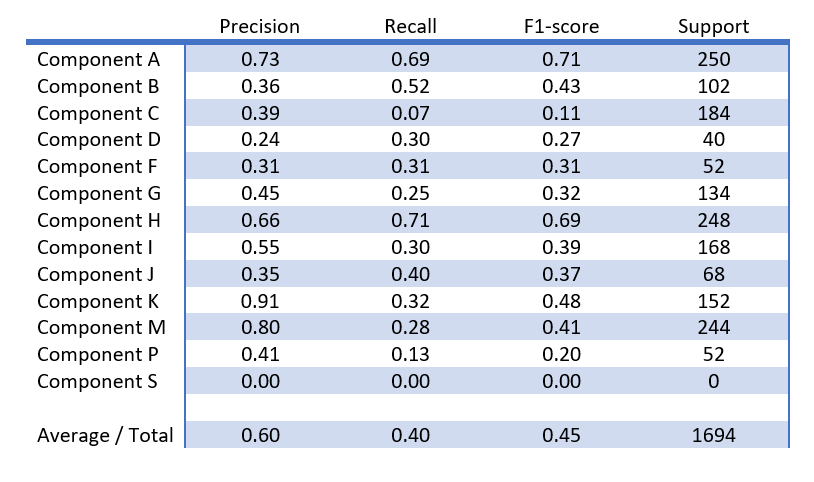
\includegraphics[width=.95\textwidth]{figures/04-go_compo_pred.PNG}
\label{fig:gocm_comp_pred}
\caption{Predicted for the Components class.}
\end{subfigure}%
}
\caption [Performance summary of the Components class trained on Inception\_v3]{These figure are the summaries of the performance for the multi-label classification trained on Inception\_v3. It shows precision, recall, f1-score and also the number of samples for each class.}
\label{fig:perf_goog}
\end{figure}

\section{Optimizer}\label{sec:opt}
\subsection{Optimization}
Based on the results of the previous experiment, we chose to optimize further Inception\_v3. Last experiment also showed that the initialization impacted the results similarly on all labels. Our hypothesis described in \ref{sec:init} is confirmed. We can focus on Dunham for the optimization.
In this experiment we tried to capture what learning rate was best for our network. We tried the following values: 0.1, 0.01 and 0.01. In Table \ref{tab:optimlr}, we summarize the results of the different learning rate. Then in Figure \ref{fig:optim_plot}, we can see the training for each learning rate. 

\begin{table}
\caption{\label{tab:optimlr} The results of training Inception network using different learning rate on the Dunham class}
\centering
\begin{tabular}[b]{| l | l | l |}
\hline
    Learning rate & Validation score  & Test score\\ \hline
    0.1  &  88,9\%  & 34,4\% \\ \hline
    0.01 & 97,1\% &  68,4\%\\ \hline
    0.001 & 85,3\% &  36,3\% \\ \hline
\end{tabular} 
\end{table}

\begin{figure}
\makebox[\linewidth][c]{%
\begin{subfigure}[b]{.6\textwidth}
\centering
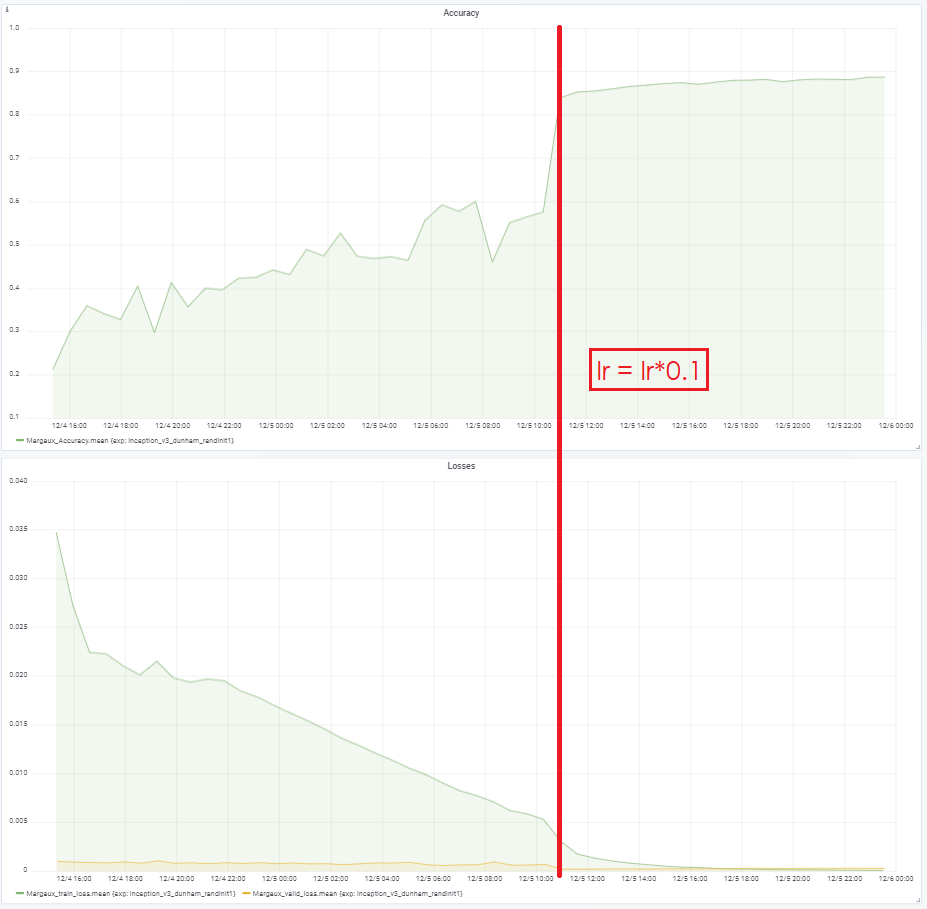
\includegraphics[width=.95\textwidth]{figures/04-opt_dunham_01.PNG}
\label{fig:optim_01}
\caption{Learning rate = 0.1}
\end{subfigure}%
\begin{subfigure}[b]{.6\textwidth}
\centering
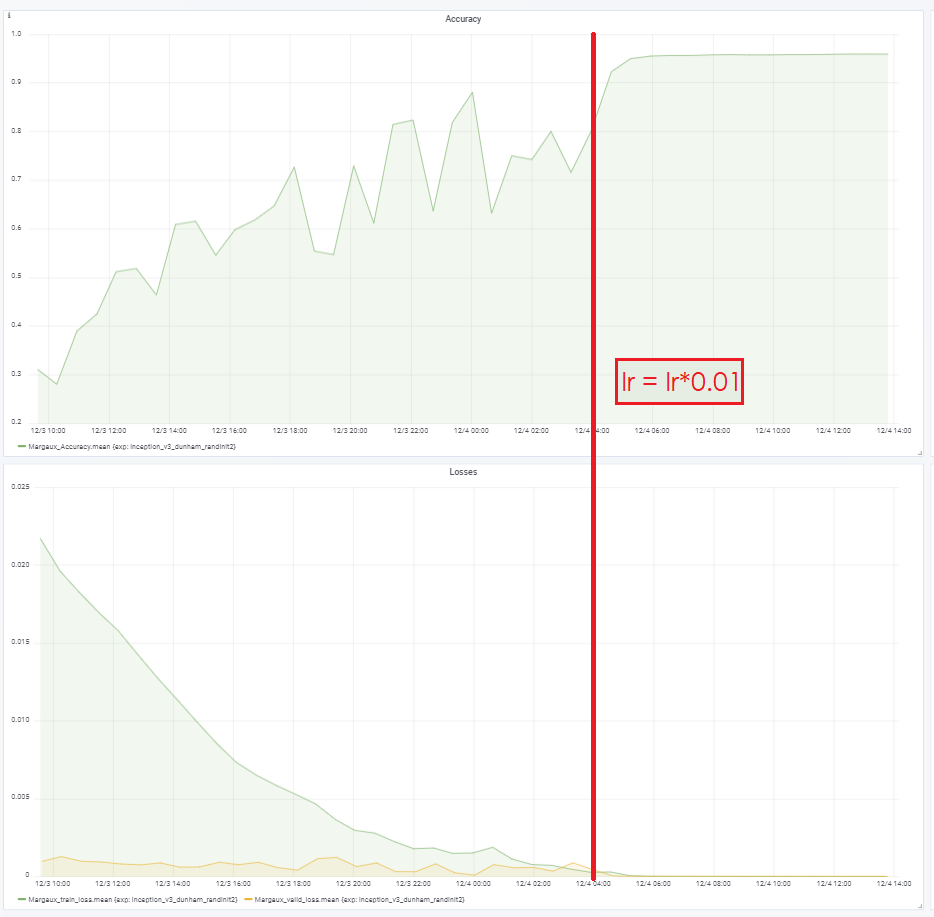
\includegraphics[width=.95\textwidth]{figures/04-opt_dunham_001.PNG}
\label{fig:optim_001}
\caption{Learning rate = 0.01}
\end{subfigure}%
}\\
\makebox[\linewidth][c]{%
\begin{subfigure}[b]{.6\textwidth}
\centering
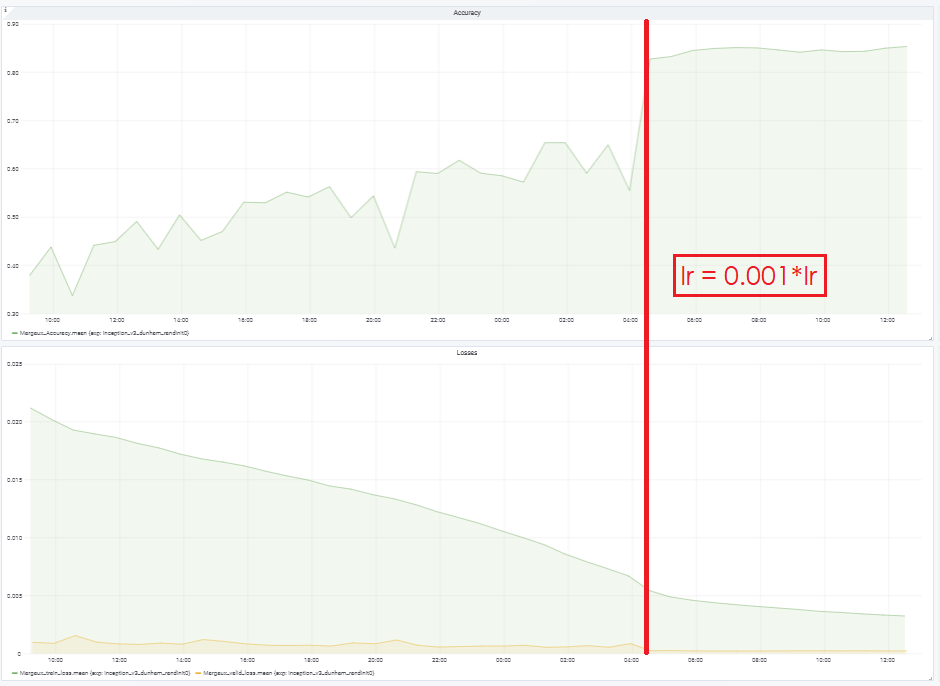
\includegraphics[width=.95\textwidth]{figures/04-opt_dunham_0001.PNG}
\label{fig:optim_1}
\caption{Learning rate = 0.001}
\end{subfigure}%
}
\caption[Training with different Learning rates]{The top plot is the validation accuracy, and the bottom plot is training (in green) and validation (in yellow) losses. Those plots are the result of training Inception\_v3 on the Dunham class for different learning rates. The red line represent when the learning rate was decayed by 0.1}
\label{fig:optim_plot}
\end{figure}


\subsection{Classification}

Finally, we applied our best performing network to all the classes. Table \ref{tab:optimall} summarizes the results obtained. In Figure \ref{fig:cm_optim}, we see the best predicted confusion matrix on the test set.  

\begin{table}
\caption{\label{tab:optimall} The results of training Inception network using 0.01 as learning rate learning rate}
\centering
\begin{tabular}[b]{| l | l | l |}
\hline
    Class & Validation score  & Test score\\ \hline
    Dunham  &  97,1\%  & 68,4\% \\ \hline
    Porosity & 95,4\% &  65,0\%\\ \hline
    DRT & 92,6\% &  24,6\% \\ \hline
    Components & 91,1\% &  40,3\% \\ \hline
\end{tabular} 
\end{table}

\begin{figure}
\makebox[\linewidth][c]{%
\begin{subfigure}[b]{.6\textwidth}
\centering
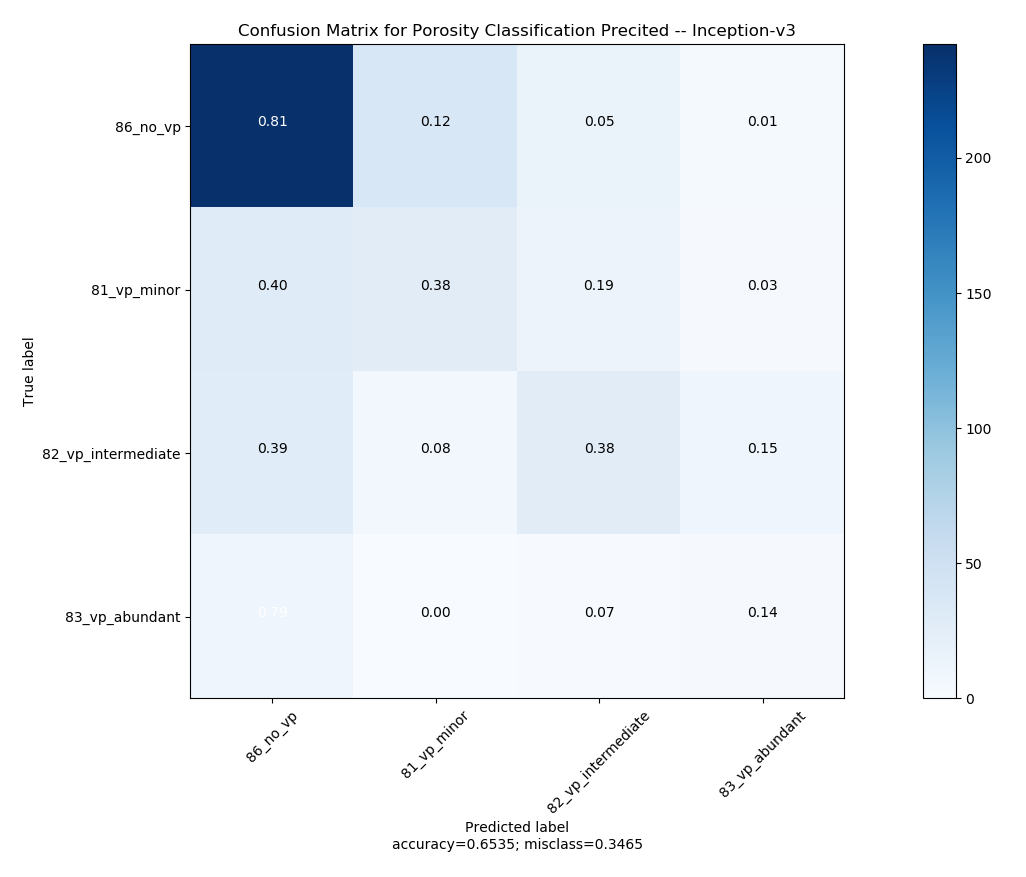
\includegraphics[width=.95\textwidth]{figures/04-norm_baby_65.PNG}
\label{fig:optcm_poro}
\caption{Predicted for Porosity}
\end{subfigure}%
\begin{subfigure}[b]{.6\textwidth}
\centering
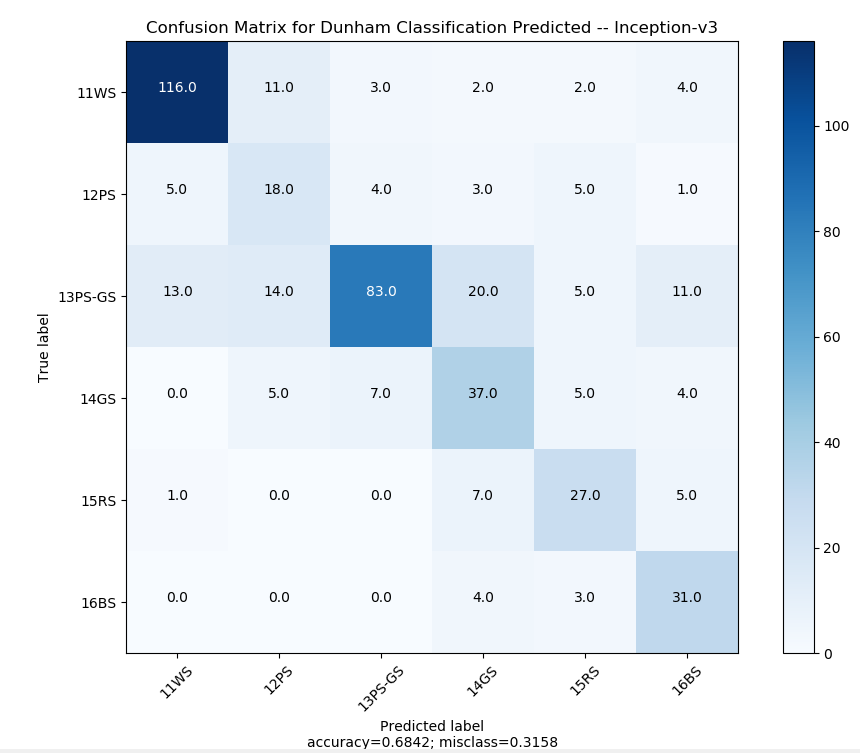
\includegraphics[width=.95\textwidth]{figures/04-dunham_69_e28.PNG}
\label{fig:optcm_dunham}
\caption{Predicted for Dunham}
\end{subfigure}%
}\\
\makebox[\linewidth][c]{%
\begin{subfigure}[b]{.6\textwidth}
\centering
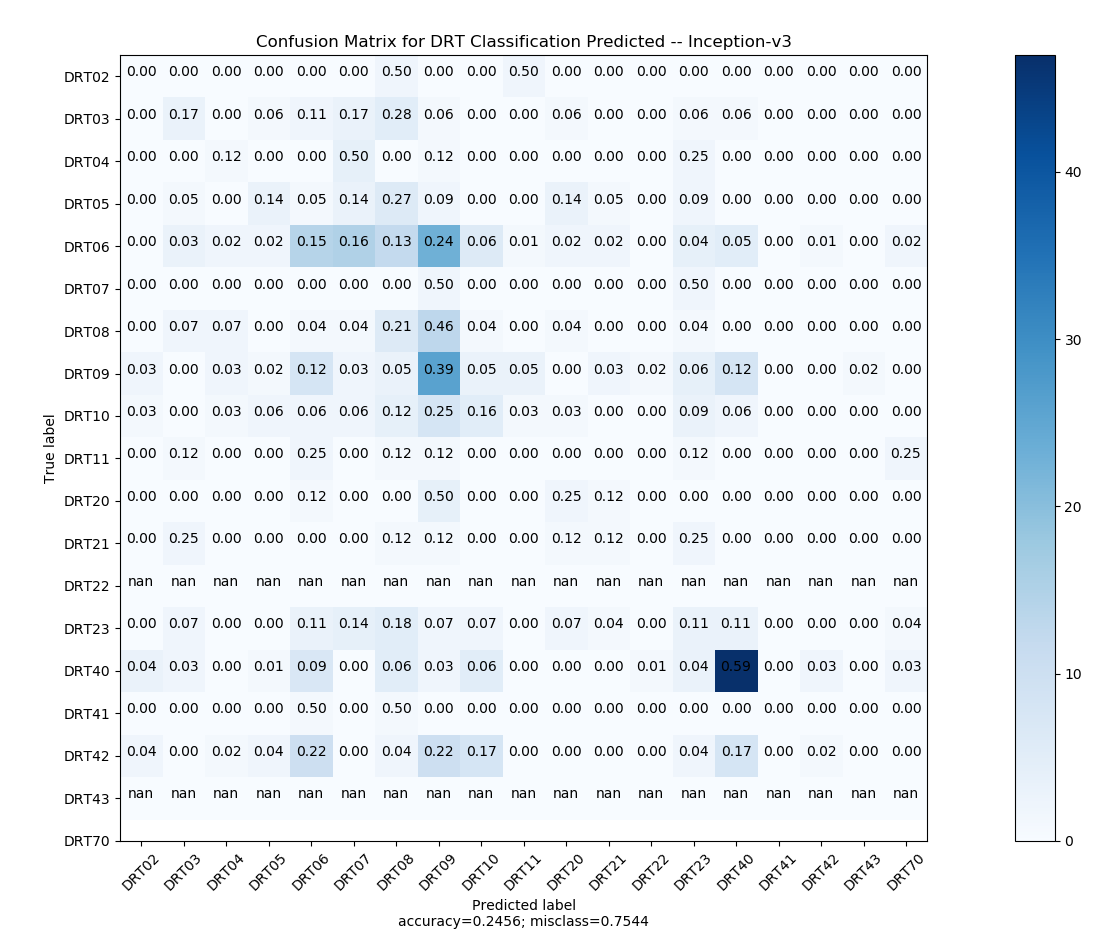
\includegraphics[width=.95\textwidth]{figures/04-norm_drt_24_e43.PNG}
\label{fig:optcm_drt}
\caption{Predicted for DRT}
\end{subfigure}%
\begin{subfigure}[b]{.6\textwidth}
\centering
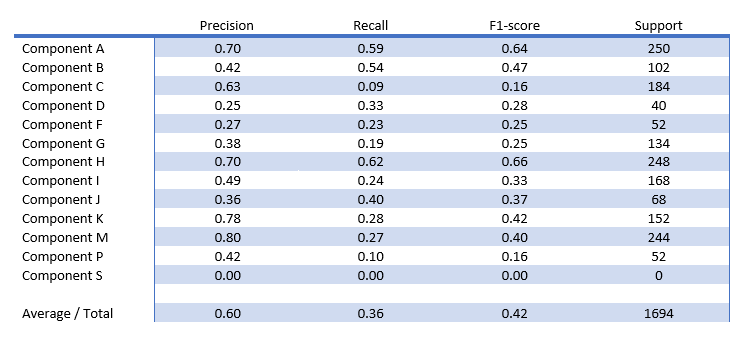
\includegraphics[width=.95\textwidth]{figures/04-compo_pred_42_e24.PNG}
\label{fig:optcm_compo}
\caption{Predicted for Components}
\end{subfigure}%
}
\caption[Confusion matrices of classes predicted with Inception\_v3]{Those figures represent the Confusion Matrix of each class on the test set. The last row contains the summary of the performance for the multi-label classification. It shows precision, recall, F1-score and also the number of samples for each class}
\label{fig:cm_optim}
\end{figure}